\chapter{曲线和方程的应用}
\section{有关求轨迹方程问题}
求轨迹（曲线）方程是解析几何的重要问题之一，求符合条件的轨迹方程的常用的一些方法介绍如下.

\subsection{直接法求轨迹方程}
已知轨迹上动点运动所遵循的几何条件，利用解析几何中的基本公式，可直接将该几何条件转化为代数形式——轨迹方程；或利用基本曲线（平面几何中的基本轨迹，以及椭圆、抛物线和双曲线等）的定义，直接写出其方程. 这就是直接法.

\begin{example}
    已知平面内有相距8个单位的两个定点$A$、$B$，求到$A$、$B$的距离之比为$1:2$的动点$P$的轨迹方程．
\end{example}

\begin{analyze}
    欲求动点的轨迹方程，需适当选取坐标系（以有利于运算为选系原则），从而确定了定点$A$、$B$的坐标，在设出动点坐标后，利用两点间距离公式，可把所给几何条件转化为方程.
\end{analyze}

\noindent
\begin{minipage}{.47\textwidth}\CTEXindent
\begin{solution}
    以$A$、$B$所在直线为$x$轴，以线段$AB$的垂直平分线为$y$轴建立坐标系．如图6.1．于是$A$，$B$坐标分别为$(-4,0)$、$(4,0)$，设动点$P$的坐标为$(x,y)$，由已知$|PA|:|PB|=1:2$，

    $\therefore\quad \frac{\sqrt{(x+4)^2+y^2}}{\sqrt{(x-4)^2+y^2}}=\frac{1}{2}$

化简得
\[3x^2+3y^2+40x+48=0\]
即为动点$P$的轨迹方程.
\end{solution}
\end{minipage}\hfill
\begin{minipage}{.5\textwidth}
    \centering
\begin{tikzpicture}[>=stealth, scale=.55]
  \draw[->](-5,0)--(5,0)node[below]{$x$};
  \draw[->](0,-2)--(0,5)node[left]{$y$};
\node[below left]{$O$};
\tkzDefPoints{-4/0/A, 4/0/B, -2/2.58/P}
\draw[very thick](A)node[below]{$A(-4,0)$}--(P)node[above]{$P(x,y)$}--(B)node[below left]{$B(4,0)$};



\end{tikzpicture}    
\captionof{figure}{}
\end{minipage}




\begin{example}
    已知$\odot O$的方程为$x^2+y^2=16$，点$A(2,0)$，动圆$P$过点$A$且与定圆$\odot O$相切，求动圆$\odot P$的圆心$P$的轨迹方程.
\end{example}

\begin{analyze}
    坐标系已建立，由于点$A$在$\odot O$内部，故$\odot P$与$\odot O$只能内切．由两圆内切的条件，即切点在连心线上，及圆心距等于大圆半径与小圆半径之差等几何性质来解决问题.
\end{analyze}


\noindent
\begin{minipage}{.57\textwidth}
\CTEXindent
\begin{solution}
如图6.2．设两圆内切于$M$，则$O$、$P$、$M$三点共线. 又$|PM|=|PA|$, $|OM|=4$,

$\therefore\quad |OP|+|PA|=|OP|+|PM|=4$.

$\therefore\quad P$点轨迹是以$O$、$A$为焦点，长轴长为4的椭圆，其中心为$(1,0)$，故其轨迹方程是
\[\frac{(x-1)^2}{4}+\frac{y^2}{3}=1\]    
\end{solution}

\end{minipage}\hfill
\begin{minipage}{.4\textwidth}
    \centering
\begin{tikzpicture}[>=stealth, scale=.45]
  \draw[->](-5,0)--(5,0)node[below]{$x$};
  \draw[->](0,-5)--(0,5)node[left]{$y$};
\node[below left]{$O$};
\draw[very thick](0,0)circle(4);
\draw[thick](1,1.732)circle(2);
\tkzDefPoints{1/1.732/P, 2/0/A, 0/0/O}
\tkzLabelPoints[below](A)
\tkzLabelPoints[left](P)
\draw(O)--(P)--(A);
\draw(P)--(60:4)node[above]{$M$};
\end{tikzpicture}    
\captionof{figure}{}
\end{minipage}

\subsection{用参数法求轨迹方程}
\noindent
\begin{minipage}{.5\textwidth}
\CTEXindent
\begin{example}
    已知定点$A(4,2)$和抛物线$y^2=4x$. 点$Q$在抛
物线上运动，动点$P$分线段$\overline{AQ}$的比为$2:1$，求$P$点的轨迹方程，并说明曲线名称.
\end{example}

\begin{analyze}
    动点$P$的位置取决于$Q$点的位置. 确定$P$点的运动规律，可以以$Q$为“参照物”，利用$Q$点坐标满足的方程来求$P$的轨迹方程. 此即以$Q$的坐标为参数.
\end{analyze}
\end{minipage}\hfill
\begin{minipage}{.45\textwidth}
    \centering
\begin{tikzpicture}[>=stealth, scale=.7]
  \draw[->](-1,0)--(6,0)node[below]{$x$};
  \draw[->](0,-4)--(0,4)node[left]{$y$};
\node[below left]{$O$};
\draw[domain=-4:4, very thick]plot({0.25*\x*\x}, \x);
\tkzDefPoints{2/2.828/Q, 4/2/A, 2.667/2.552/P}
\draw(Q)node[left]{$Q(x_1,y_1)$}--(A)node[right]{$A(4,2)$};
\tkzDrawPoints(A,Q,P)
\node at(P)[above right]{$P(x,y)$}; 
\end{tikzpicture}    
\captionof{figure}{}
\end{minipage}

\begin{solution}
如图6.3，设$P(x,y)$，$Q(x_1,y_1)$

$\because\quad P$分$\overline{AQ}$的比为$2:1$,

$\therefore\quad \begin{cases}
    x=\frac{4+2x_1}{1+2}\\[1.5ex]
    y=\frac{2+2y_1}{1+2}
\end{cases}$
解出
$\begin{cases}
    x_1=\frac{3x-4}{2}\\[1.5ex] y_1=\frac{3y-2}{2}
\end{cases}$

把$x_1,y_1$代入方程$y^2=4x$，从而消去$x_1,y_1$. 即
    \[\left(\frac{3y-2}{2}\right)^2=4\cdot \frac{3x-4}{2}\]
    化简得：$$\left(y-\frac{2}{3}\right)^2=\frac{8}{3}\left(x-\frac{4}{3}\right)$$
    其轨迹是以$\left(\frac{4}{3},\frac{2}{3}\right)$为顶点，其轴平行$x$轴，开口向右的一条抛物线.
\end{solution}

\begin{example}
    已知，如图6.4，$\odot O$的方程为$x^2+y^2=4$，$\odot O$与$x$轴正半轴交于$A$，$M$为圆上任意一点，$BM\parallel OX$, $BM$交$y$轴于$B$，直线$OM$与$AB$交于$P$.

求动点$P$的轨迹方程.
\end{example}

\begin{analyze}
    当$M$位置确定后，点$B$随之确定，从而直线$OM$
    和$AB$也确定，由此$P$点位置可确定. 总之$P$点位置决定于$M$点的位置. 因此可选点$M$为“参照物”，即设$M$的坐标为参数，可利用$M$在已知$\odot O$上的条件解决问题.
\end{analyze}

\begin{solution}   
 \textbf{解法1：} 设$P(x,y)$, $M(x_1,y_1)$，则$B(0,y_1)$.

 \noindent
 \begin{minipage}{.5\textwidth}
 \CTEXindent
 
 由于$O$、$P$、$M$三点共线，$A$、$P$、
$B$三点共线，

$\therefore\quad \begin{cases}
   \frac{y}{x}= \frac{y_1}{x_1}\\[1.5ex]
   \frac{y-0}{y_1-0}=\frac{x-2}{0-2}
\end{cases}$

解之得
$\begin{cases}
    x_1=\frac{-2x}{x-2}\\[1.5ex] 
    y_1=\frac{-2y}{x-2}
\end{cases}$

$\because\quad (x_1,y_1)$在$\odot O$上，

$\therefore\quad x_1^2+y_1^2=4$.

化简得$y^2=-4(x-1),\quad (y\ne 0)$

上式为所求的轨迹方程.
 \end{minipage}\hfill
 \begin{minipage}{.47\textwidth}
     \centering
 \begin{tikzpicture}[>=stealth, scale=1.05]
   \draw[->](-3,0)--(3,0)node[below]{$x$};
   \draw[->](0,-3)--(0,3)node[left]{$y$};
 \node[below left]{$O$};
 
 \draw[very thick](0,0) circle(2);
 \tkzDefPoints{0/0/O, 2/0/A, 0/1/B}
 \tkzDefPoint(30:2){M}
\tkzLabelPoints[left](B)
\tkzLabelPoints[right](M)
\tkzLabelPoints[below right](A)
\draw(A)--(B)--(M)--(O) ;
\tkzInterLL(A,B)(O,M) \tkzGetPoint{P}
\tkzLabelPoints[below](P)
 \end{tikzpicture}    
 \captionof{figure}{}
 \end{minipage}

\textbf{解法2：}由$M$在$\odot O$上，可利用圆的参数方程．设点$M$的坐标为$(2\cos\theta, 2\sin\theta)$，则$B(0,2\sin\theta)$．

可得$OM$方程为$y=x\cdot \tan\theta$（$\theta$为参数），
$AB$方程为$y=-\sin\theta (x-2)$.

消去参数$\theta$，即得$P$点轨迹方程
\[y=-2\x2 \left(x-\frac{2}{2}\right)=-4(x-1)\]
    
\end{solution} 

\begin{example}
    已知椭圆$\frac{x^2}{a^2}+\frac{y^2}{b^2}=1\; (a>b>0)$. 求斜率为$k\; (k\ne 0)$的平行弦的中点的轨迹方程（图6.5）．
\end{example}




\noindent
\begin{minipage}{.47\textwidth}
\begin{analyze}
\textbf{分析1：} 斜率为$k$的弦所在直线方程可用直线系$y=kx+m\; (m\in\R)$表示，则方程组$\begin{cases}
    \frac{x^2}{a^2}+\frac{y^2}{b^2}=1 \\ y=kx+m
\end{cases}$的解是直线与椭
圆交点的坐标. 显然交点坐标是$m$的函数. 由线段中点坐标公式，可求得弦中点的参数方程（$m$为参数），进而可求得普通方程.
\end{analyze}
\end{minipage}\hfill
\begin{minipage}{.5\textwidth}
    \centering
\begin{tikzpicture}[>=stealth]
  \draw[->](-3,0)--(3,0)node[below]{$x$};
  \draw[->](0,-2)--(0,2)node[left]{$y$};
\node[below right]{$O$};
\draw(0,0)ellipse(2.5 and 1.5);

\foreach \m in {.8, 2.4, -2.4, -.8}
{
    \draw[domain={(12.5*\m+sqrt(478.125-56.25*\m*\m))/17}:{(12.5*\m-sqrt(478.125-56.25*\m*\m))/17}, thick]plot(\x, {-\x+\m});
    \tkzDefPoint({(12.5*\m+sqrt(478.125-56.25*\m*\m))/17},{-(12.5*\m+sqrt(478.125-56.25*\m*\m))/17+\m}){A}
    \tkzDefPoint({(12.5*\m-sqrt(478.125-56.25*\m*\m))/17},{-(12.5*\m-sqrt(478.125-56.25*\m*\m))/17+\m}){B}
    \tkzDefMidPoint(A,B) \tkzGetPoint{C}
    \tkzDrawPoints(C)
}
\node at (A)[below right]{$P_1(x_1,y_1)$};
\node at (B)[above left]{$P_2(x_2,y_2)$};
\node at (C)[below]{$P(x,y)$};
\draw[domain=2.14:-2.14]plot(\x, 0.36*\x);
\tkzDrawPoint(2.14,.77)
\tkzDrawPoint(-2.14,-.77)



\end{tikzpicture}    
\captionof{figure}{}
\end{minipage}





\begin{solution}
 \textbf{解法1：}设斜率为$k$的弦所在直线方程为
\begin{equation}
    y=kx+m  \tag{1}
\end{equation}
代入椭圆方程，消$y$，化简得
\begin{equation}
    (b^2+a^2k^2)x^2+2a^2kmx+a^2m^2-a^2b^2=0 \tag{*}
\end{equation}

$\because\quad $直线与椭圆交于两点，

$\therefore\quad \Delta =(2a^2km)^2-4(b^2+a^2k^2)(a^2m^2-a^2b^2)>0$，
化简得
\[|m|<\sqrt{a^2k^2+b^2}\]
又直线与椭圆交点的横坐标，恰为方程(*)的两个解$x_1$和$x_2$，设弦的中点为$(x,y)$，则
$x=\frac{x_1+x_2}{2}$，即
\begin{equation}
    x=\frac{-a^2km}{b^2+a^2k^2} \tag{2}
\end{equation}

由(1)(2)消去$m$，得
\[y=\frac{-b^2}{a^2 k}x,\quad x\in\left(-\frac{a^2|k|}{\sqrt{a^2k^2+b^2}},\; \frac{a^2|k|}{\sqrt{a^2k^2+b^2}}\right)\]

此即椭圆$\frac{x^2}{a^2}+\frac{y^2}{b^2}=1\; (a>b>0)$中斜率为$k$的弦的中点轨迹方程.
\end{solution}

\begin{analyze}
\textbf{分析2：}
 由于轨迹上的点是椭圆的斜率为$k$的弦的中点，所以也可直接设出弦的端点坐标$A(x_1,y_1)$、$B(x_2,y_2)$，再利用$AB$的中点公式及过两点的直线的斜率公式来解决.
\end{analyze}

\begin{solution}
\textbf{解法2：}设弦的端点为$A(x_1,y_1)$, $B(x_2,y_2)$.

$\because\quad A$、$B$是椭圆上的点，

$\therefore\quad \begin{cases}
    \frac{x_1^2}{a^2}+\frac{y_1^2}{b^2}=1\\
    =1
\end{cases}$两式相减，得
\[ \frac{x_1^2}{a^2}-\frac{x_2^2}{a^2}+\frac{y_1^2}{b^2}-\frac{y_2^2}{b^2} =0\]
即
\begin{equation}
    b^2(x_1+x_2)(x_1-x_2)+a^2(y_1+y_2)(y_1-y_2)=0 \tag{**}
\end{equation}

设弦$AB$的中点为$P(x,y)$, 则$x=\frac{x_1+x_2}{2}$, $y=\frac{y_1+y_2}{2}$

又$AB$的斜率$k=\frac{y_2-y_1}{x_2-x_1}$，代入方程(**)，得
\[b^2\cdot 2x(x_1-x_2)+a^2\cdot 2y\cdot k(x_1-x_2)=0\]
即
\[y=-\frac{b^2}{a^2k}x\]

可求得直线$y=-\frac{b^2}{a^2k}x$与椭圆交点的横坐标为$\pm\frac{a^2|k|}{\sqrt{a^2k^2+b^2}}$

故弦中点轨迹为线段$y=-\frac{b^2}{a^2k}x\quad \left(|x|<\frac{a^2|k|}{\sqrt{a^2k^2+b^2}}\right)$
\end{solution}

\begin{remark}
解法2通常称之为“多参法”，即设曲线上的两点坐标$x_1,y_1,x_2,y_2$为参数，而后消去这些参数，得出所求轨迹方程，对于二次曲线中平行弦的中点轨迹问题较为简便.
\end{remark}

\noindent
\begin{minipage}{.4\textwidth}\CTEXindent
    \begin{example}
        一条没有弹性的细绳绕在一个圆面完全固定的圆盘的侧面上. 当绳的外端拉紧逐渐展开时，使展开的部分拉直随时都成为圆的切线（图6.6）．这样，绳的外端点的轨迹叫做\textbf{圆的渐开线}. 这个圆叫做渐开线的\textbf{基圆}.
        
        试求圆的渐开线的方程.
        \end{example}
\end{minipage}\hfill
\begin{minipage}{.57\textwidth}
    \centering
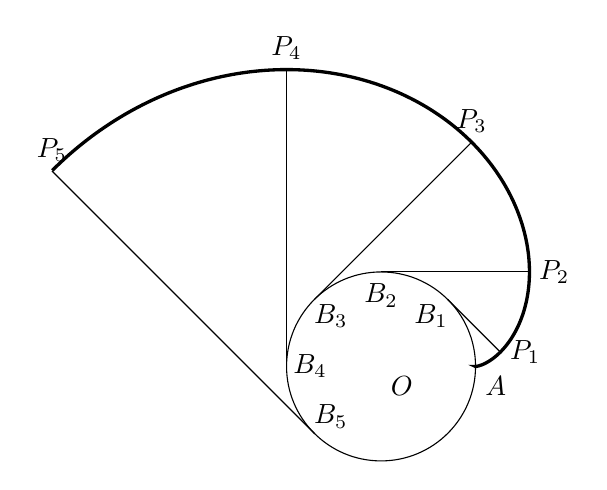
\begin{tikzpicture}[>=stealth, scale=1.2]

\draw(0,0)node[below right]{$O$}circle(1);

\foreach \x in {1,2,...,5}
{
    \node at (45*\x:.75){$B_{\x}$};
}
\tkzDrawPoint(0,0)
\node at (1,0)[below right]{$A$};


\tkzDefPoints{0/0/O}

\foreach \x in {1,2}
{
    \draw(45*\x:1)--+(45*\x-90:.785*\x)node[right]{$P_{\x}$};
}
\foreach \x in {3,4,5}
{
    \draw(45*\x:1)--+(45*\x-90:.785*\x)node[above]{$P_{\x}$};
}
\draw[domain=0:1.25*pi, smooth, very thick, samples=1000]plot({cos(\x r)+\x*sin(\x r)}, {sin(\x r)-\x*cos(\x r)});
\end{tikzpicture}    
\captionof{figure}{}
\end{minipage}



\begin{analyze}
设$\odot O$的半径为$r$，细绳外端的初始位置为$A$. 以$O$为原点，有向直线$OA$为$x$轴，建立坐标系（图6.7）．设曲线上的动点为$P(x,y)$. $BP$是圆的切线，$B$为切点，连结$OB$，显然$P$点位置取决于$B$点的位置，由于$P$点运动的规律是$\wideparen{AB}\text{的长}=|BP|$，而$\wideparen{AB}$的长与$\wideparen{AB}$所对的角$\angle AOB$有直接关系，因此若设
$\angle AOB=\varphi$为参数，则可找到$P$点坐标与$B$点坐标之间的联系，即可列出其参数方程.
\end{analyze}

\begin{solution}
建立坐标系如图6.7.

设$P(x,y)$，$B(x_1,y_1)$，$BP$是圆的切线，$B$为切点.

设$\angle AOB=\varphi$（弧度数）是以$OA$为始边，以$OB$为终边的正角，由已知$|BP|=\wideparen{AB}\text{的长}=r\varphi$，$x_1=r\cos\varphi$，$y_1=r\sin\varphi$.

过$B$作$BC\bot OA$于$C$，过$P$作$PD\bot BC$于$D$，则$\angle PBD=\varphi$
于是
\[\begin{cases}
    x=x_1+|BP|\sin\varphi\\
    y=y_1-|BP|\cos\varphi
\end{cases}\]
即
\[\begin{cases}
    x=r(\cos\varphi+\varphi\sin\varphi)\\
    y=r(\sin\varphi-\varphi\cos\varphi)
\end{cases}\text{（$\varphi$为参数）}\]
此即圆的渐开线的参数方程.
\end{solution}


\noindent
\begin{minipage}{.57\textwidth}
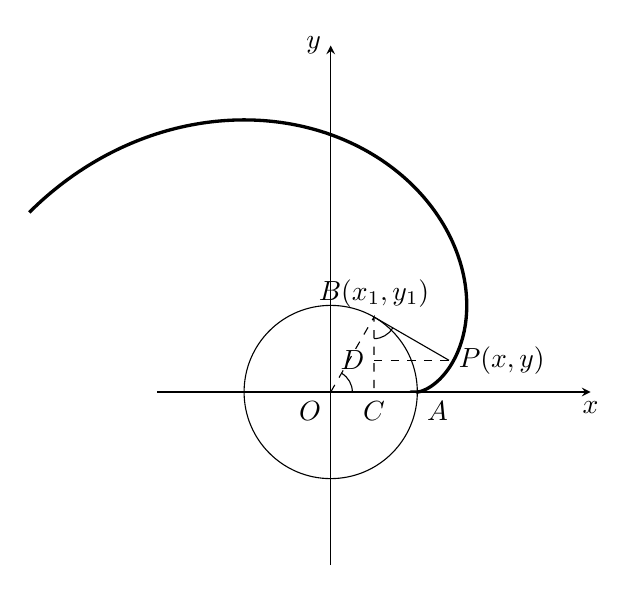
\begin{tikzpicture}[>=stealth, scale=1.1]
  \draw[->](-2,0)--(3,0)node[below]{$x$};
  \draw[->](0,-2)--(0,4)node[left]{$y$};
\node[below left]{$O$};
\draw(0,0)circle (1);
\draw[domain=0:1.25*pi, smooth, very thick, samples=1000]plot({cos(\x r)+\x*sin(\x r)}, {sin(\x r)-\x*cos(\x r)});
\draw(60:1)node[above]{$B(x_1,y_1)$}--+(-30:1)node[right]{$P(x,y)$};
\draw[dashed](0,0)--(60:1)--(.5,0)node[below]{$C$};
\draw[dashed](.5,.866-.5)node[left]{$D$}--+(.866,0);
\node at (1,0)[below right]{$A$};
\draw(.25,0) arc (0:60:.25);
\draw(.5,.866-.25)arc (-90:-30:.25);

\end{tikzpicture}    

\captionof{figure}{}
\end{minipage}\hfill
\begin{minipage}{.47\textwidth}
    \centering
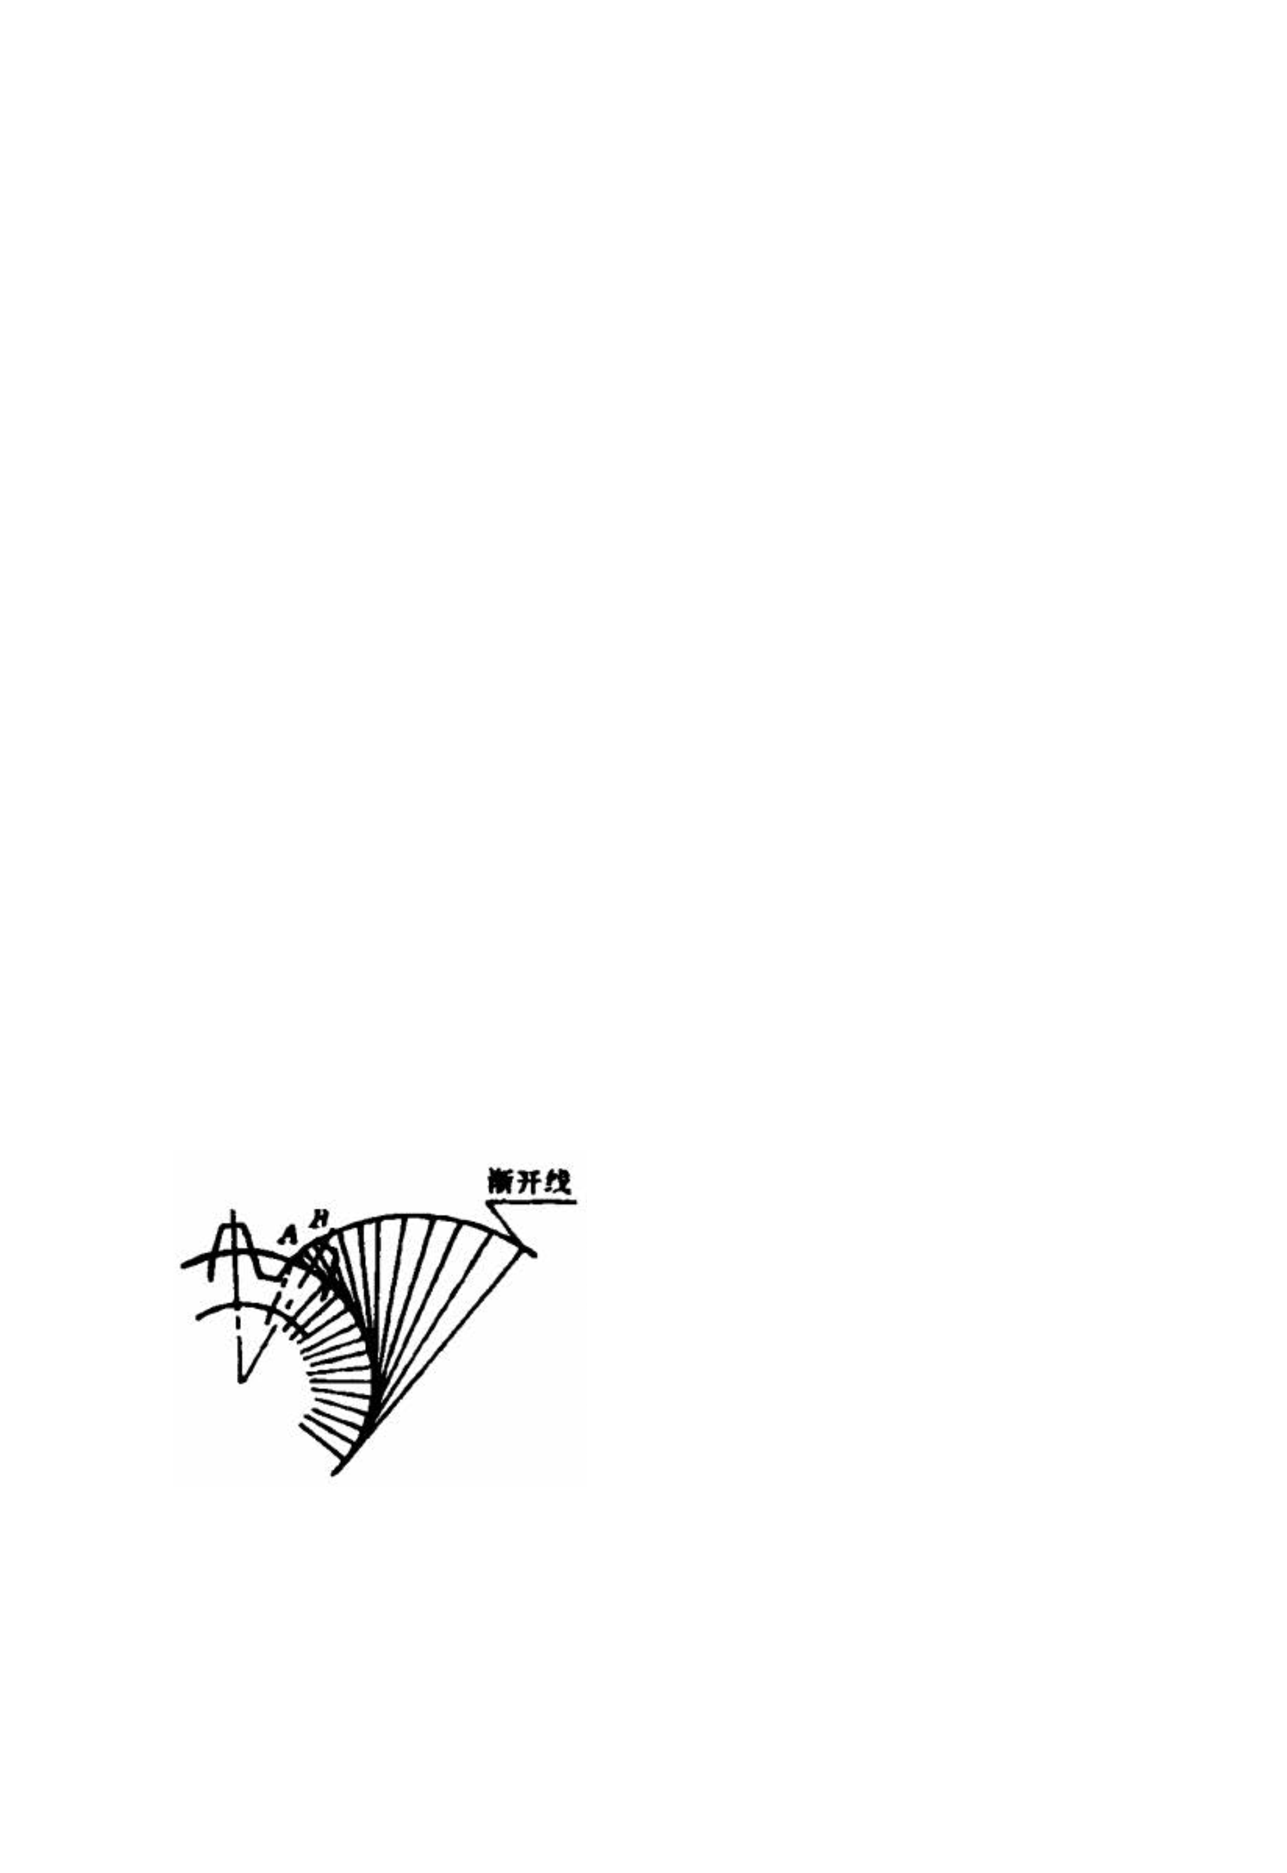
\includegraphics[scale=.8]{fig/6-8.pdf}
\captionof{figure}{}
\end{minipage}




在机械上，广泛应用着齿轮传递动力，大多数齿轮采用渐开线齿形（图6.8）．这种齿轮磨损小，传动平稳，制造安装也较为方便.设计加工这种齿轮，就需要用到圆的渐开线方程.

\begin{example}
一个圆沿着一条定直线
滚动时，圆周上的一个定点的轨迹
叫旋轮线（图6.9）．

试求旋轮线的方程.
\end{example}

\begin{figure}[htp]
    \centering
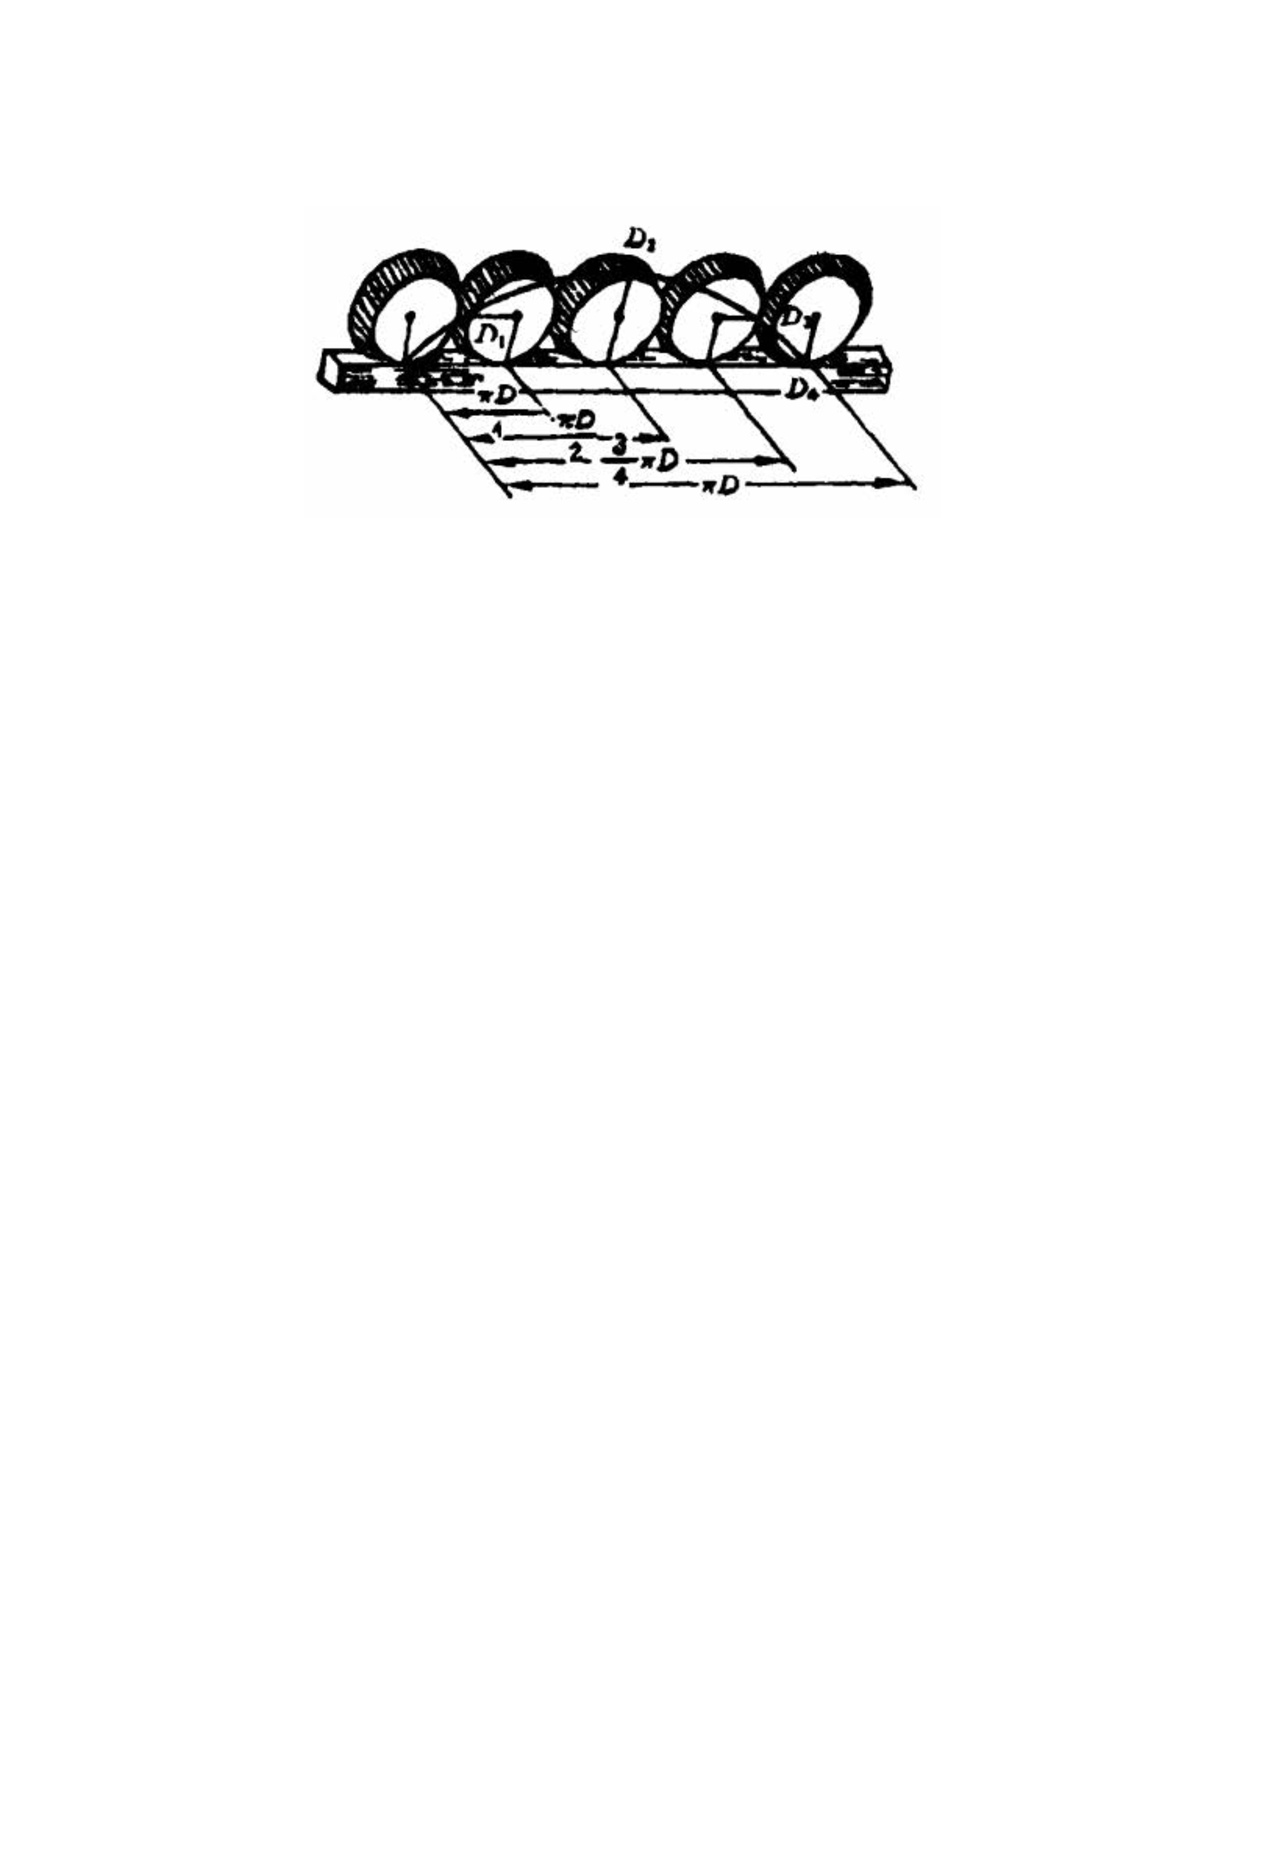
\includegraphics[scale=.8]{fig/6-9.pdf}
    \caption{}
\end{figure}

\begin{solution}
设圆的半径为$r$，圆上的定点为$P$，取点$P$与定直线初始接触点为原点$O$，定直线为$x$轴，建立坐标系（图6.10）.
\begin{figure}[htp]
    \centering
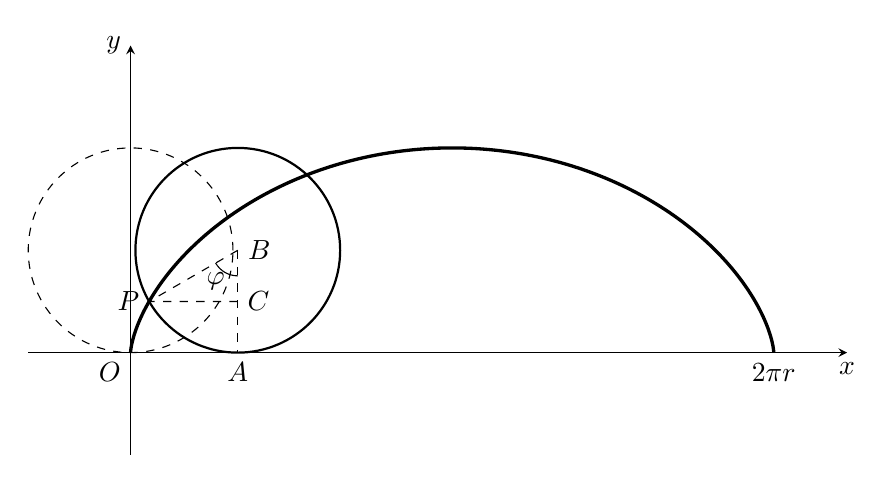
\begin{tikzpicture}[>=stealth, scale=1.3]
    \draw[->](-1,0)--(7,0)node[below]{$x$};
    \draw[->](0,-1)--(0,3)node[left]{$y$};
  \node[below left]{$O$};
\draw[dashed](0,1)circle(1);
\draw[thick](pi/3,1)node[right]{$B$}circle(1);
\draw[dashed](pi/3,1)--(pi/3,0)node[below]{$A$};
\draw[dashed](pi/3,1)--+(-150:1)node[left]{$P$}--(pi/3,.5)node[right]{$C$};
\draw[domain=0:2*pi,smooth, samples=100, very thick]plot({\x-sin(\x r)}, {1-cos(\x r)})node[below]{$2\pi r$};
\draw(pi/3,1-.25) arc (-90:-150:.25)node[below]{$\varphi$};

\end{tikzpicture}
    \caption{}
\end{figure}

当圆沿$x$轴方向滚动，圆心位于$B$点（此时，圆与$x$轴相切于点$A$，定点移至图中$P$点标出的位置）时，显然有
\[|OA|=\wideparen{PA}\text{的长}\]

不难看出：点$P$的位置取决于点$B$的位置，而点$B$的坐标$(x_1,y_1)$可由圆心角$\angle ABP=\varphi$（弧度数）表示：
\[\begin{cases}
    x_1=|OA|=\wideparen{AP}=r\varphi\\
y_1=r
\end{cases}\]

过$P$作$PC\bot BA$于$C$，则
\[|PC|=r\sin\varphi,\qquad |BC|=r\cos\varphi\]
所以
\[\begin{cases}
    x=x_1-|PC|=r\varphi-r\sin\varphi\\
    y=y_1-|BC|=r-r\cos\varphi\\
\end{cases}\]
即\[\begin{cases}
    x=r(\varphi-\sin\varphi)\\
    y=r(1-\cos\varphi)
\end{cases}\text{（$\varphi$为参数）}\]

这就是旋轮线的参数方程.
\end{solution}

当圆滚动一周，即$\varphi$从0变到$2\pi$时，点$P$描出曲线的第一拱．圆再向前滚动一周，即$\varphi$从$2\pi$变到$4\pi$时，点$P$描出曲线的第二拱. 显然，第二拱的形状和第一拱完全相同. 圆继续向前滚动，可得第三拱、第四拱、…… 圆向后滚动的情况也是一样. 可见旋轮线是由无数段拱形弧组成的，拱宽为$2\pi r$，拱高为$2r$．

旋轮线有不少重要性质. 例如，质点在重力作用下从点$A$滑落到点$B$（假定无磨擦），当下滑的曲线是什么形状时所需的时间最短（这就是所谓“最速降线问题”）？答案是：曲线是一条翻转的旋轮线（图6.11）
（这个结论用微积分可以证明）. 因此，旋轮线又叫\textbf{最速降线}.


\noindent
\begin{minipage}{.47\textwidth}
    \centering
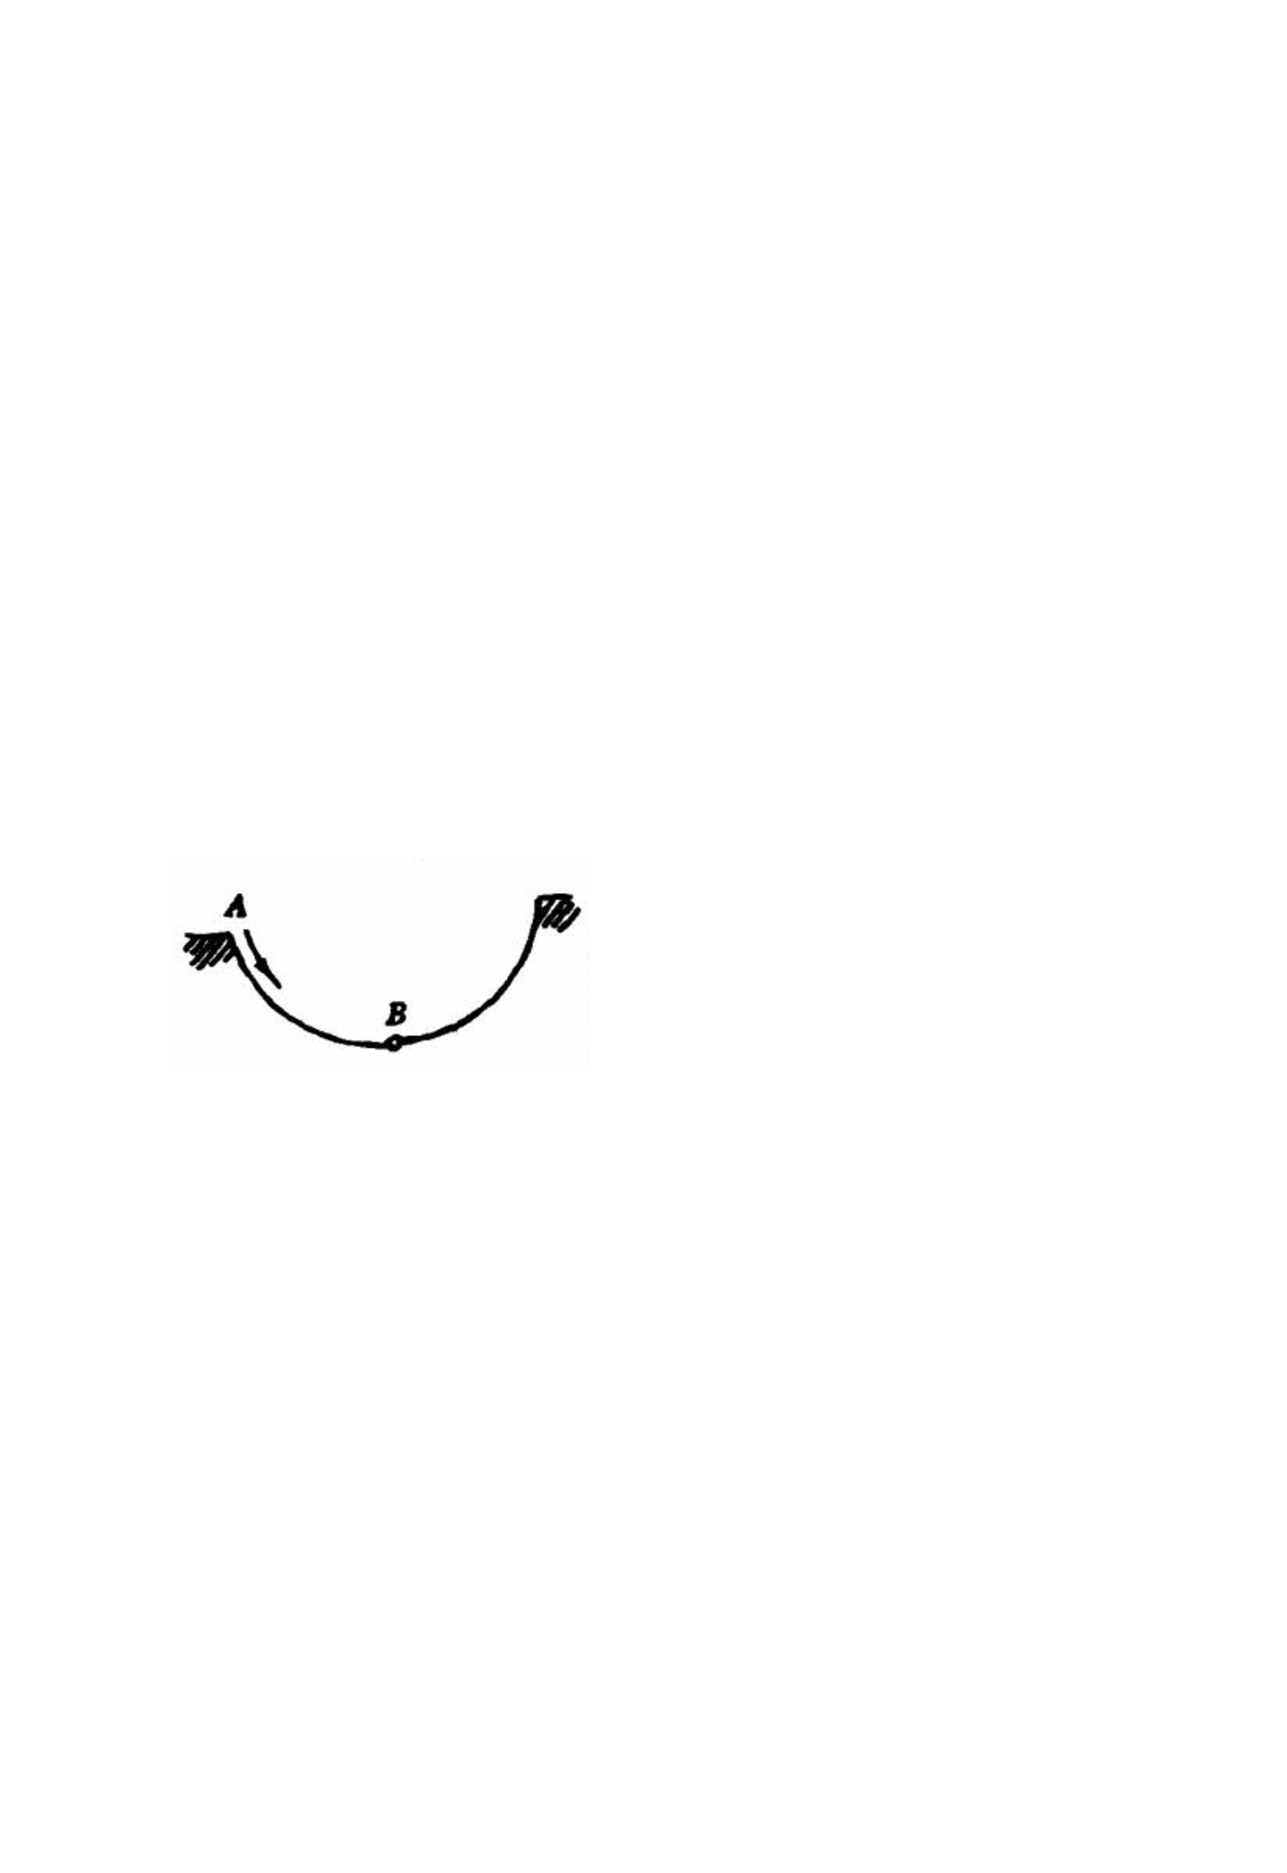
\includegraphics[scale=.7]{fig/6-11.pdf}
\captionof{figure}{}
\end{minipage}\hfill
\begin{minipage}{.47\textwidth}
    \centering
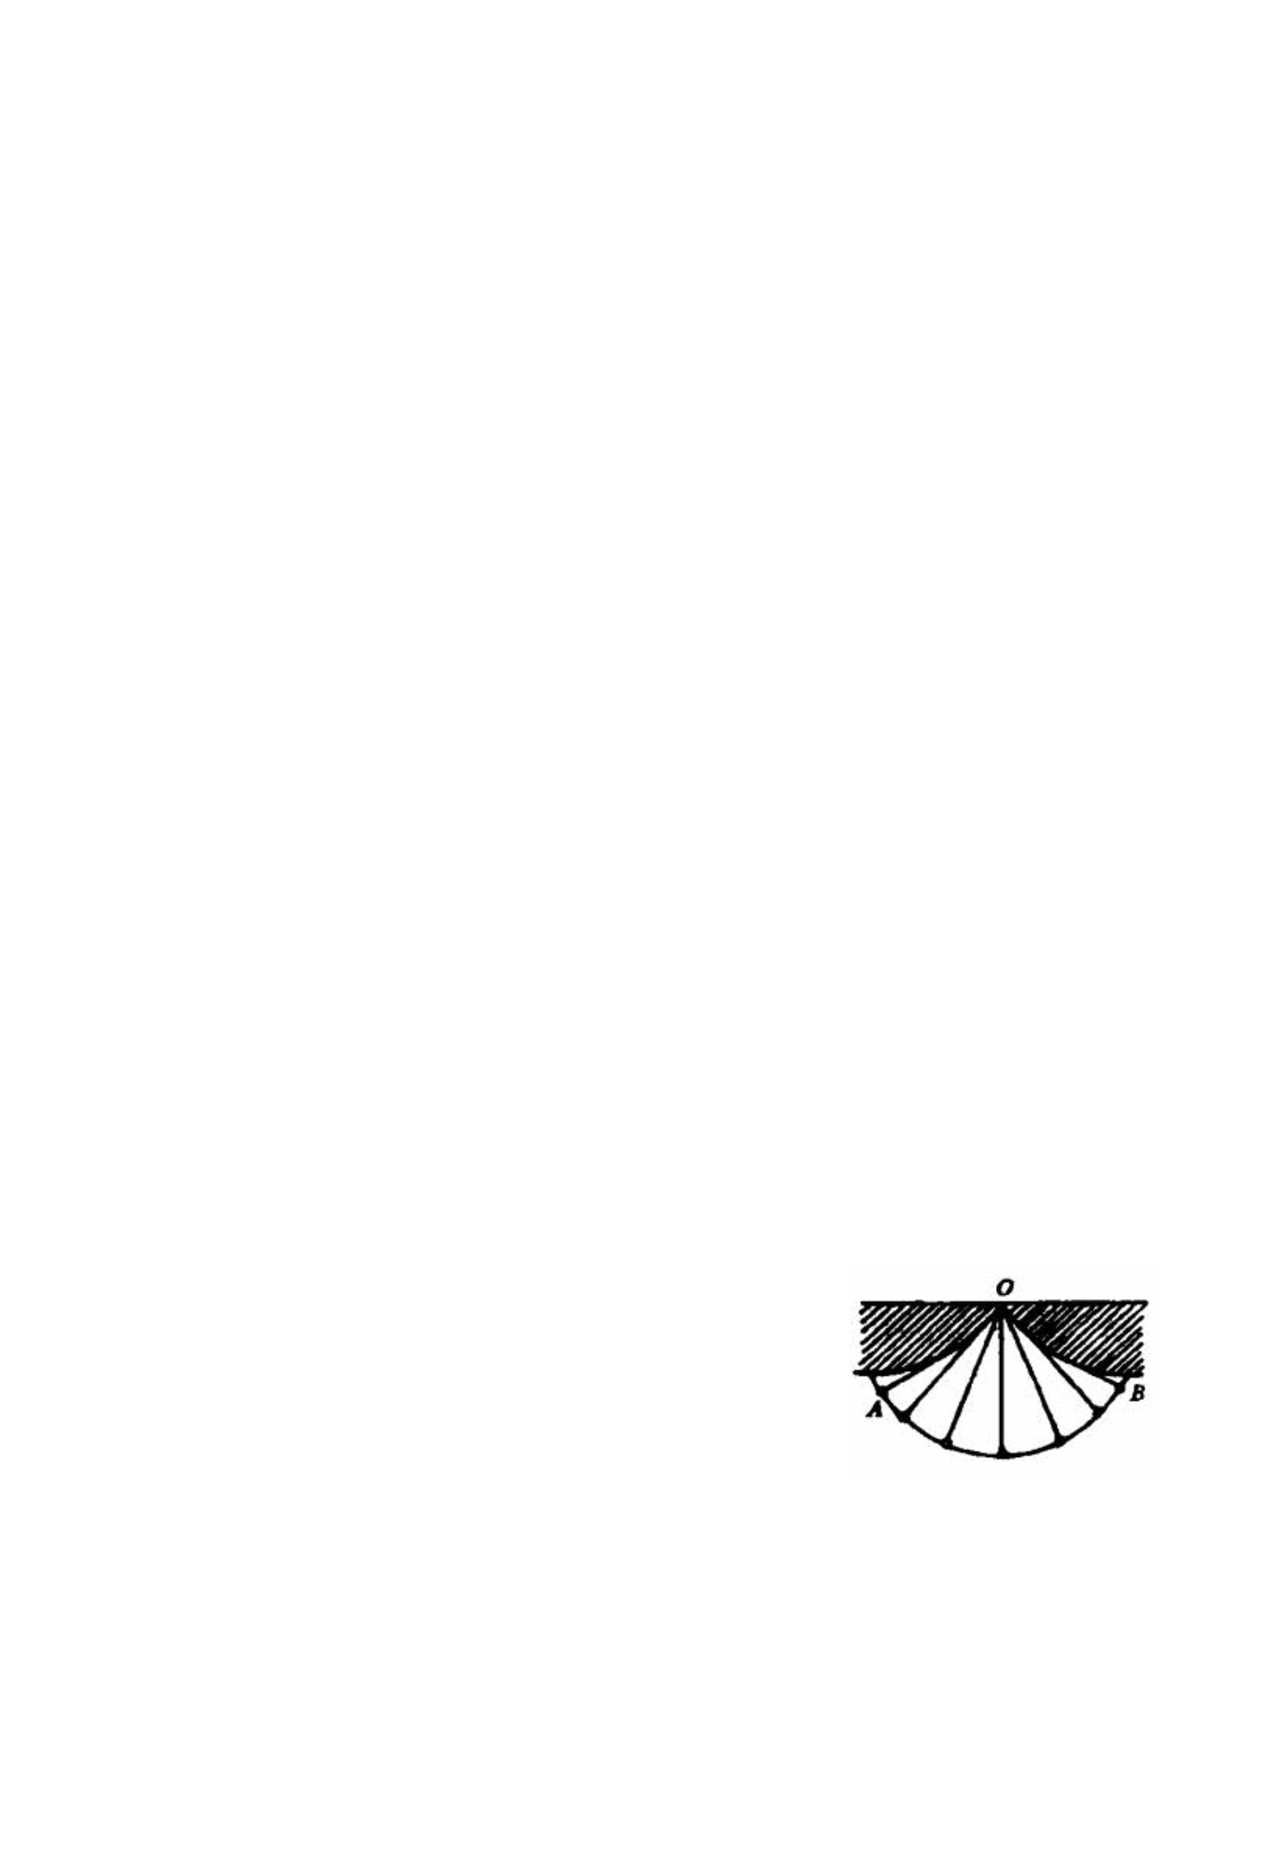
\includegraphics[scale=.7]{fig/6-12.pdf}
\captionof{figure}{}
\end{minipage}

又如，普通单摆的摆动周期与振幅大小有关，如果在摆动平面内做两个旋轮线形状的挡板（图6.12中的$OA$与$OB$），这样，摆的运动轨迹将也是一条旋轮线，而摆动周期将与振幅大小无关.在17世纪，旋轮线即以此性质出名，所以又称为\textbf{摆线}.


\subsection*{6.1 练习}
\begin{enumerate}
    \item 求经过定点$M(1,2)$，以$y$轴为准线，离心率为$\frac{1}{2}$的椭圆左顶点的轨迹方程.
    \item 已知椭圆$\frac{x^2}{a^2}+\frac{y^2}{b^2}=1\; (a>b>0)$及点$P(2a,0)$，点$Q$在椭圆上运动，求$PQ$中点$M$的轨迹方程.
\item 已知动点$P$到椭圆$\frac{x^2}{a^2}+\frac{y^2}{b^2}=1\; (a>b>0)$的长轴两端点的距离之积，等于它到短轴两端点的距离之积，求动点$P$的轨迹方程.
\item 已知$A$是椭圆$\frac{(x+2)^2}{4}+\frac{(y-1)^2}{3}=1$上任意一点，$B$是定点$(0,4)$，动点$P$分线段$\overline{AB}$的比为$1:2$，求$P$点的轨迹方程.
\item 在双曲线$x^2-y^2=4$中，求斜率为2的平行弦的中点的轨迹方程.
\item 在抛物线$y^2=2px\; (p>0)$中，求斜率为$k$的平行弦的中点轨迹方程.
\end{enumerate}

\section{有关证明问题}
\begin{example}
已知椭圆$\frac{x^2}{a^2}+\frac{y^2}{b^2}=1\; (a>b>0)$，$P(x_0,y_0)$为椭圆上的任意一点（异于椭圆顶点），连结$P$与椭圆短轴端点$B_1$、$B$的直线分别交$x$轴于$M$和$N$．（如图6.13）

求证：$|OM|\cdot |ON|$为定值.
\end{example}

\begin{figure}[htp]
    \centering
\begin{tikzpicture}[>=stealth]
    \draw[->](-3,0)--(5,0)node[below]{$x$};
    \draw[->](0,-2)--(0,2)node[left]{$y$};
\draw[thick](0,0)node[below left]{$O$} ellipse (2 and 1);
\tkzDefPoints{0/0/O, 4/0/A, 0/1/B, 0/-1/B_1, 1.5/.661/P}
\tkzInterLL(B_1,P)(O,A) \tkzGetPoint{M}
\tkzInterLL(B,P)(O,A) \tkzGetPoint{N}
\tkzDrawSegments[very thick](B_1,P B,N)
\tkzLabelPoints[below](M,N)
\tkzLabelPoints[below left](B_1)
\tkzLabelPoints[above left](B)
\node at (P)[above right]{$P(x_0,y_0)$};


\end{tikzpicture}
    \caption{}
\end{figure}

\begin{analyze}
    $|OM|$与$|ON|$分别为$M$和$N$的横坐标的绝对值，因此首先应求出直线$B_1P$和$BP$与$x$轴交点的坐标，再利用$P$为椭圆上的点的条件进行证明.
\end{analyze}

\begin{proof}
    设$M(m,0)$, $N(n,0)$, $B_1(0,-b)$, $B(0,b)$.

$\because\quad     B$、$P$、$N$三点共线，$B_1$、$M$、$P$三点共线，

$\therefore\quad \begin{cases}
    \frac{0-b}{n-0}=\frac{y_0-b}{x_0-0}\\[1.5ex]
    \frac{0+b}{m-0}=\frac{y_0+b}{x_0-0}
\end{cases}$解之得：$\begin{cases}
    n=\frac{-bx_0}{y_0-b}\\[1.5ex]
    m=\frac{bx_0}{y_0+b}\\
\end{cases}$

$\because\quad (x_0,y_0)$在椭圆上 

$\therefore\quad b^2x^2_0+a^2y^2_0=a^2b^2$，因此：
\[|OM|\cdot |ON|=|mn|=\left|\frac{b^2x^2_0}{y^2_0-b^2}\right|=\frac{|a^2b^2-a^2y^2_0|}{|y^2_0-b^2|}=a^2\]
\end{proof}

\begin{remark}
椭圆上的点$P(x_0,y_0)$的坐标满足椭圆方程是证明过程中的关键之一.
\end{remark}

\begin{example}
过抛物线$y^2=2px$的顶点$O$，任意作两条互相垂直的弦$OA$和$OB$（如图6.14）．连结$AB$．

求证：弦$AB$必过定点，并求出这个定点的坐标.
\end{example}


\noindent
\begin{minipage}{.57\textwidth}
\begin{analyze}
可通过建立直线$AB$的方程说明这些直线过定点，显然需要找出$A$、$B$的坐标. $A$、$B$的坐标可通过设出直线$OA$和$OB$的方程与抛物线方程联立，求出$A$、$B$坐标；也可通过直接设出$A$、$B$坐标，再通过$OA\bot OB$的条件来寻求其间的关系，最终得出$AB$的直线系方程，进而证明其直线系过定点. 另一方面由于抛物线关于$x$轴对称，由此可推断，该定点必在$x$轴上.
\end{analyze}
\end{minipage}\hfill
\begin{minipage}{.4\textwidth}
    \centering
\begin{tikzpicture}[>=stealth, scale=.8]
  \draw[->](-1,0)--(5,0)node[below]{$x$};
  \draw[->](0,-3)--(0,3)node[left]{$y$};
\node[below left]{$O$};
\draw[domain=2.7:-2.7, thick, samples=100, smooth]plot({.5*\x*\x}, \x);
\tkzDefPoints{0/0/O, 3.125/2.5/A, 1.28/-1.6/B}
\tkzDrawPolygon(A,B,O)
\tkzLabelPoints[below](B)
\tkzLabelPoints[above](A)
\tkzMarkRightAngles[size=.2](A,O,B)
\end{tikzpicture}    
\captionof{figure}{}
\end{minipage}

\begin{solution}
\textbf{解法1：} 设$OA$方程为$y=kx$，则$OB$方程为$y=-\frac{1}{k}x$. 由此知$A\left(\frac{2p}{k^2},\; \frac{2p}{k}\right)$, $B(2pk^2,-2pk)$，则$AB$的方程为
\[\left(\frac{2p}{k^2}-2pk^2\right)\left(y-\frac{2p}{k}\right)=\left(\frac{2p}{k}+2pk\right)\left(x-\frac{2p}{k^2}\right)\]
令$y=0$，得$x=2p$. 即直线$AB$过定点$(2p,0)$.

\textbf{解法2：}设$A\left(\frac{y^2_1}{2p},\; y_1\right)$, $B\left(\frac{y^2_2}{2p},\; y_2\right)$

$\because\quad OA\bot OB$,

$\therefore\quad \frac{y_1}{\frac{y^2_1}{2p}}\cdot \frac{y_2}{\frac{y^2_2}{2p}}=-1$
可得$y_1y_2=-4p^2$.

又当$y_1\ne -y_2$时，$AB$方程可写为
\[y-y_1=\frac{2p}{y_1+y_2}\left(x-\frac{y^2_1}{2p}\right)\]
即$(y_1+y_2)y-y_1^2-y_1y_2=2px-y_1^2$.

令$y=0$，及$y_1y_2=-4p^2$，得$x=2p$. 即$AB$过定点$(2p,0)$.

\textbf{解法3：}利用抛物线的参数方程，设点$A(2pt_1^2,2pt_1)$，
$B(2pt_2^2, 2pt_2)$. 设$AB$与$x$轴交点为$M(x_0,0)$.

$\because \quad OA\bot OB$

$\therefore\quad \frac{2pt_1}{2pt_1^2}\cdot \frac{2pt_2}{2pt_2^2}=-1\quad \Rightarrow\quad  t_1\cdot t_2=-1$

又$A$、$B$、$M$共线，

$\therefore\quad \frac{2pt_1-0}{2pt^2_1-x_0}=\frac{2pt_1-2pt_2}{2pt_1^2-2pt_2^2},\quad \frac{2pt_1}{2pt_1^2-x_0}=\frac{1}{t_1+t_2}$

$\therefore\quad 2pt_1(t_1+t_2)=2pt^2_1-x_0 \quad \Rightarrow \quad x_0=-2pt_1t_2$

$\therefore\quad x_0=2p$，即$AB$过定点$M(2p,0)$.
\end{solution}



\noindent
\begin{minipage}{.55\textwidth}

\begin{example}
已知椭圆$\frac{x^2}{a^2}+\frac{y^2}{b^2}=1\; (a>b>0)$，$F_1,F_2$为其焦点，$P$是椭圆上的一点，设$\angle F_1PF_2=\alpha$（图6.15）.

求证：$\triangle PF_1F_2$的面积$S=b^2\tan\frac{\alpha}{2}$.
\end{example}

\begin{analyze}
$S_{\triangle PF_1F_2}=\frac{1}{2}|PF_1|\cdot |PF_2|\sin\alpha$. 可利用椭圆定义知$|PF_1|+|PF_2|=2a$，及三角形中的正弦定理或余弦定理来
解决问题.
\end{analyze}
\end{minipage}\hfill
\begin{minipage}{.43\textwidth}
    \centering
\begin{tikzpicture}[>=stealth]
  \draw[->](-2.5,0)--(2.5,0)node[below]{$x$};
  \draw[->](0,-2)--(0,2)node[left]{$y$};
\node[below left]{$O$};
\draw[thick](0,0)ellipse(2 and 1);

\tkzDefPoints{1.732/0/F_2, -1.732/0/F_1, 1.5/0.66/P}
\tkzLabelPoints[below](F_1,F_2)
\tkzLabelPoints[above](P)
\draw[very thick](F_1)--(P)--(F_2);
\end{tikzpicture}    
\captionof{figure}{}
\end{minipage}

\begin{proof}
$\because\quad |PF_1|+|PF_2|=2a, \quad |F_1F_2|=2c$

$\therefore\quad |PF_1|^2+|PF_2|^2+2|PF_1|\cdot |PF_2|=4a^2$ \hfill(1)

又由余弦定理有
\begin{equation}
   |PF_1|^2+|PF_2|^2-2|PF_1|\cdot |PF_2|\cos\alpha=4c^2  \tag{2}
\end{equation}

(1)(2)相减，得
\[2|PF_1|\cdot |PF_2|(1+\cos\alpha)=4a^2-4c^2\]

$\therefore\quad \frac{1}{2}|PF_1|\cdot |PF_2|=\frac{a^2-c^2}{1+\cos\alpha}=\frac{b^2}{1+\cos\alpha}$

$\therefore\quad S_{\triangle PF_1F_2}=\frac{1}{2}|PF_1|\cdot |PF_2|\sin\alpha=\frac{b^2\sin\alpha}{1+\cos\alpha}=b^2\tan\frac{\alpha}{2}$.
\end{proof}

\subsection*{6.2 练习}
\begin{enumerate}
\item 证明：过点$P(a\cos^3\alpha, a\sin^3\alpha)$且与直线$x\sec\alpha+y\csc\alpha=a$垂直的直线方程是$x\cos\alpha-y\sin\alpha=a\cos2\alpha$.
\item 证明：等轴双曲线上任意一点到中心的距离是它到两个焦点距离的比例中项.
\item 设抛物线的轴与它的准线相交于点$A$，经过焦点垂直于轴的直线交抛物线于$B$、$C$两点，求证：$BA\bot CA$.
\item 过定点的直线与抛物线$y^2=2px$交于$M$、$N$两点，求证：$M$与$N$的横坐标之积、纵坐标之积都是常数.
\item 求证：双曲线的渐近线与准线的交点到其中心的距离等于实半轴的长；焦点到渐近线的距离等于虚半轴的长.
\end{enumerate}

\section{有关最小值和最大值问题}
解析几何中常见的一些最小值和最大值问题，通常利用曲线的定义、几何性质或利用函数及平均不等式来解决.

\noindent
\begin{minipage}{.57\textwidth}
    \begin{example}
        在抛物线$y^2=4x$上求一点$P$，使得$P$到定点$A(4,2)$与抛物线的焦点$F$的距离之和最小，并求出该最小值（图6.16）．
    \end{example}

\begin{analyze}
如果设$P$点坐标为$\left(\frac{y^2}{4},y\right)$，再求$|PA|+|PF|$和的最小值，将是极为繁琐的. 如果考虑到抛物线的定义，即抛物线上任意一点到焦点的距离等于其到准线的距离，如图中的$|P'F|=|P'H'|$，便有$|P'A|+|P'F|=|P'A|+|P'H'|$，则当$A$、$P'$、$H'$三点在一条直线上时其和最短. 问题便成为非常简单的事情.
\end{analyze}

\end{minipage}\hfill
\begin{minipage}{.4\textwidth}
    \centering
\begin{tikzpicture}[>=stealth, scale=.7]
  \draw[->](-2,0)--(5,0)node[below]{$x$};
  \draw[->](0,-4.5)--(0,4.5)node[left]{$y$};
\node[below left]{$O$};
\draw[domain=3.7:-3.7, thick, samples=100, smooth]plot({.25*\x*\x}, \x);
\tkzDefPoints{4/2/A, 1/0/F, -1/2/H, 2/2.828/P', -1/2.828/H', -1/4/L, 1/2/P}
\draw(-1,4)--(-1,-3.5)node[left]{$\ell$};
\tkzLabelPoints[right](A)
\tkzLabelPoints[below](F,P)
\tkzLabelPoints[above](P')
\tkzLabelPoints[left](H,H')
\draw[very thick](A)--(P')--(H');
\draw[very thick](A)--(P)--(H);
\draw[very thick](P')--(F);
\tkzMarkRightAngles[size=.2](L,H',P' L,H,P)


\end{tikzpicture}    
\captionof{figure}{}
\end{minipage}

\begin{solution}
过$A$作$AH$垂直于准线，垂足为$H$，$AH$交抛物线于$P$，则$|PA|+|PF|$取得最小值，此时$P(1,2)$，最小值为5.
\end{solution}

\begin{remark}
    充分注意曲线的定义是使问题解决得到简化的重要因素.
\end{remark}


\noindent
\begin{minipage}{.5\textwidth}
\begin{example}
已知椭圆$\frac{x^2}{16}+\frac{y^2}{9}=1$及点$A(4,0)$、$B(0,3)$在椭圆上，求一点$P$，使得$\triangle PAB$的面积最大，并求出该最大值（图6.17）．
\end{example}

\begin{analyze}
\textbf{分析1：}欲使$S_{\triangle PAB}$最大，只需$P$到直线$AB$的距离最大. 由此可写出$AB$的方程. 设$P(a,b)$，通过求$P$到$AB$的距离的最大值，求出$P$的坐标.
\end{analyze}
\end{minipage}\hfill
\begin{minipage}{.48\textwidth}
    \centering
\begin{tikzpicture}[>=stealth, scale=.5]
  \draw[->](-6,0)--(6,0)node[below]{$x$};
  \draw[->](0,-5)--(0,5)node[left]{$y$};
\node[below left]{$O$};
\draw[thick](0,0) ellipse(4 and 3);
\tkzDefPoints{4/0/A, -4/0/A', 0/3/B, 0/-3/B', -3/-1.98/P}

\tkzLabelPoints[above left](B)
\tkzLabelPoints[below right](A)
\tkzLabelPoints[below left](A',B',P)
\tkzDrawPolygon[very thick](A,P,B)
\end{tikzpicture}    
\captionof{figure}{}
\end{minipage}



\begin{solution}
\textbf{解法1：}$AB$的方程为$3x+4y-12=0$.

设$P(a,b)$，则$P$到$AB$的距离为
\[d=\frac{|3a+4b-12|}{5}\]

由于$P$在椭圆上，且只有当$P$在第三象限时，$d$才能取得最大值. 于是可用$a$表示$b$，使$d$化为$a$的一元函数. 有
\[\begin{split}
    d&=\frac{1}{5}\left|3a+4\left(-\frac{3}{4}\sqrt{16-a^2}\right)-12\right|\\
    &=\frac{3}{5}\left|-a+\sqrt{16-a^2}+4\right|
\end{split}\]
其中
\[\begin{split}
    \sqrt{16-a^2}-a&=\sqrt{16-a^2+a^2-2a\sqrt{16-a^2}}\\
    &=\sqrt{16+2\sqrt{a^2(16-a^2)}}
\end{split}\]
当且仅当$a^2=16-a^2$，即$a=-2\sqrt{2}$时，取得最大值$\sqrt{16+2\x8}=4\sqrt{2}$

故当$P$为$\left(-2\sqrt{2},\; -\frac{3}{2}\sqrt{2}\right)$时，$d_{\max}=\frac{12}{5}\left(\sqrt{2}+1\right)$.

此时$S_{\triangle PAB}$的最大值为$6(\sqrt{2}+1)$.
\end{solution}


\begin{analyze}
\textbf{分析2：}     若在椭圆上任取一点$P'$，过$P'$作平行于$AB$的直线$\ell$，则$P$到$AB$的距离就是$\ell$与$AB$的距离，故当$\ell$与椭圆相切时，才能使该距离最大，其切点就是所求的点.
\end{analyze}

\begin{solution}
\textbf{解法2：}$AB$方程为$3x+4y-12=0$.

设直线$\ell:\; 3x+4y+c=0$，得$4y=-3x-c$.

代入椭圆方程，消去$y$化简得
\[18x^2+6cx+c^2-144=0\]
令$\Delta =36c^2-4\x18(c^2-144)=0$，得$c=\pm 12\sqrt{2}$.

由图可知，$P$点在第三象限时符合条件.

$\therefore\quad $取$c=12\sqrt{2}$即切线为$3x+4y+12\sqrt{2}=0$.

此时该线到$AB$的距离为$\frac{12}{5}(\sqrt{2}+1)$

所求$P$点坐标为$P\left(-2\sqrt{2},\; -\frac{3}{2}\sqrt{2}\right)$.

最大面积为$6(\sqrt{2}+1)$.
\end{solution}

\begin{remark}
  把点线距离转化为平行线间距离，又利用直线与椭圆相切的条件来解决问题，与解法1比较，既减少了运算量，也好操作.
\end{remark}


\begin{analyze}
   \textbf{分析3：}若利用椭圆的参数方程，可将求点线距离问题转化为求三角式的最值问题，将给问题的解决带来方便.
\end{analyze}

\begin{solution}
\textbf{解法3：}设点$P(4\cos\theta, 3\sin\theta)$，
$AB$方程为$3x+4y-12=0$. 
$P$到$AB$的距离为
\[\begin{split}
  d=\frac{|12\cos\theta+12\sin\theta-12|}{5}&=\frac{12}{5}|\cos\theta+\sin\theta-1|\\
  &\frac{12}{5}\left|\sqrt{2}\sin\left(\theta+\frac{\pi}{4}\right)-1\right|  
\end{split}\]

$\therefore\quad $当$\theta+\frac{\pi}{4}=\frac{3}{2}\pi$时，$d_{\max}=\frac{12}{5}\left(\sqrt{2}+1\right)$，此时$P\left(-2\sqrt{2},\; -\frac{3}{2}\sqrt{2}\right)$

$S_{\triangle PAB}$的最大值为$6(\sqrt{2}+1)$.
\end{solution}

\begin{remark}
利用正弦（余弦）函数的性质，解决某些最值问题，是重要的途径之一.
\end{remark}

\begin{example}
已知椭圆$C:\; \frac{x^2}{25}+\frac{y^2}{16}=1$及直线$\ell:\; x+y-9=0$. 求与椭圆$C$有相同焦点，且与直线$\ell$有公共点的椭圆中，长轴最短的椭圆方程.
\end{example}

\noindent
\begin{minipage}{.47\textwidth}
\CTEXindent


\begin{analyze}
显然，在所有椭圆中与直线只有一个公共点的椭圆满足要求.只有一个公共点，即直线为椭圆的切线，可利用一元二次方程的判别式为0来解决问题，但运算过程将是繁琐的.

如果设$P$为所求椭圆与直线的公共点，$F_1,F_2$为椭圆焦点，则$|PF_1|+|PF_2|$就是椭圆的长轴长. 因此问题转化为在直线上求点$P$，使$|PF_1|+|PF_2|$取最小值的问题.
\end{analyze}

\end{minipage}\hfill
\begin{minipage}{.5\textwidth}
    \centering
\begin{tikzpicture}[>=stealth, scale=.3]
  \draw[->](-7,0)--(12,0)node[below]{$x$};
  \draw[->](0,-5)--(0,13)node[left]{$y$};
\node[below left]{$O$};
\draw(0,0)ellipse (5 and 4);
\tkzDefPoints{-3/0/F_1, 3/0/F_2, 9/6/F'}
\draw[domain=-3:11, thick]plot(\x, -\x+9)node[below]{$\ell$};
\tkzDefPoints{0/9/A1, 9/0/A2}
\tkzInterLL(F_1,F')(A1,A2) \tkzGetPoint{P}
\tkzInterLL(F_2,F')(A1,A2) \tkzGetPoint{P1}
\draw[thick](F_1)--(F')--(F_2);
\tkzLabelPoints[above](P,F')
\tkzLabelPoints[below](F_1,F_2)

\end{tikzpicture}    
\captionof{figure}{}
\end{minipage}

\begin{solution}
    已知 椭圆焦点为$F_1(-3,0)$、$F_2(3,0)$，可求得$F_2(3,0)$关于$\ell:\; x+y-9=0$的对称点为$F'(9,6)$，如图6.18．则$F_1F'$与$\ell$的交点$P$使得$|PF_1|+|PF_2|$最小，$|F_1F'|$就是所求椭圆的长轴长，$|F_1F'|=6\sqrt{2}$

故所求椭圆为$\frac{x^2}{18}+\frac{y^2}{9}=1$.
\end{solution}

\begin{example}
    已知矩形$ABCD$的顶点$A$、$B$在曲线$\begin{cases}
        x=4\cos2\theta \\ y=4\sqrt{2}\cos\theta
    \end{cases}$（$\theta$为参数）上运动，$C$、$D$在直线$x+y-4=0$
上运动．求矩形面积的最大值（图6.19）．
\end{example}

\begin{analyze}
 矩形面积等于$|AB|\cdot |AD|$，由于$A$的运动使得$|AB|$及$|AD|$都在变化. 但只要$A$点确定，则$|AB|$、$|AD|$随之而定，而$A$的位置的确定可由直线$AB$的方程来确定. 直线$AB$的斜率为$-1$，故可设$AB$的方程为$x+y+m=0$，其中$m$为参数. 于是可将矩形面积表示为$m$的函数，进而可求出其最大值.
\end{analyze}

\begin{solution}
  曲线$\begin{cases}
    x=4\cos2\theta \\ y=4\sqrt{2}\cos\theta
\end{cases}$（$\theta$为参数）化为普通方程就是


\noindent
\begin{minipage}{.5\textwidth}\CTEXindent
\begin{equation}
     y^2=4(x+4) \tag{1}
\end{equation}
    其中$x\in [-4,4]$, $y\in\left[-4\sqrt{2},4\sqrt{2}\right]$，即曲线是抛物线上的一段弧；

又$\because\quad $直线$CD$过点$(0,4)$，斜率为$-1$，

$\therefore\quad AB$只能在$CD$的下方（如图6.19），且$AB\parallel CD$.

设$AB$方程为$x+y+m=0$\hfill(2)

(2)代入(1)消去$y$，得
\[x^2+(2m-4)x+m^2-16=0\]
由$\Delta>0$得：$-4\le m<5$.
\end{minipage}\hfill
\begin{minipage}{.47\textwidth}
    \centering
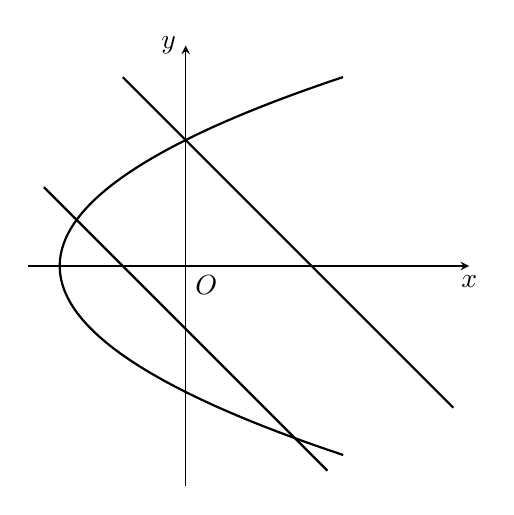
\begin{tikzpicture}[>=stealth, scale=.4]
  \draw[->](-5,0)--(9,0)node[below]{$x$};
  \draw[->](0,-7)--(0,7)node[left]{$y$};
\node[below right]{$O$};
\draw[domain=-6:6, thick, smooth, samples=100]plot({.25*\x*\x-4}, \x);
\draw[domain=-2:8.5, thick]plot(\x, -\x+4);
\draw[domain=-4.5:4.5, thick]plot(\x, -\x-2);
\tkzDefPoints{0/4/E, 4/0/F, 3.464/-5.464/B, -3.464/1.464/A}
\tkzLabelPoints[below](A,B)
\tkzDefPointBy[projection = onto E--F](A) \tkzGetPoint{D}
\tkzDefPointBy[projection = onto E--F](B) \tkzGetPoint{C}
\tkzLabelPoints[above](C,D)
\tkzDrawSegments[thick](A,D B,C)
\end{tikzpicture}    
\captionof{figure}{}
\end{minipage}

可求出$|AB|$和$|AD|$的值分别为
\[|AB|=4\sqrt{2}\cdot \sqrt{5-m},\qquad |AD|=\frac{|0+4+m|}{\sqrt{2}}\]
\[\begin{split}
\therefore\quad S_{ABCD}=|AB|\cdot |AD|&=4\sqrt{2}\cdot \sqrt{5-m}\cdot\frac{|4+m|}{\sqrt{2}}\\
&=4\sqrt{(5-m)(4+m)^2}\\
&=2\sqrt{2(10-2m)(4+m)(4+m)}
\end{split}\]

由平均不等式可知，当且仅当$m=2$时，此式有最大值$24\sqrt{3}$.
\end{solution}

\begin{example}
已知椭圆$\frac{x^2}{a^2}+\frac{y^2}{b^2}=1\; (a>b>0)$与$y$轴正半轴交于$B$点，$P$是椭圆上任意一点（异于$B$），过$P$作$PD\bot y$轴于$D$. 将$\triangle BPD$绕$y$轴旋转一周得到一个圆锥（图6.20）．

求该圆锥体积的最大值，及体积最大时$P$点的坐标.
\end{example}

\begin{analyze}
    圆锥体积决定于$P$的位置. 可设出$P$的坐标，而后将圆锥体积表示为$P$的坐标的函数，最后便可求出体积最大值. $P$点坐标的设法可用$(x_1,y_1)$，也可利用椭圆的参数方程.
\end{analyze}

\begin{solution}
    \textbf{解法1：}
设$P(a\cos\theta,b\sin\theta)$，则
\[|PD|=|a\cos\theta|,\quad |BD|=b-b\sin\theta\quad \text{（$\theta$为参数）}\]
\[\begin{split}
    \text{圆锥体积}V&=\frac{1}{3}\pi (a\cos\theta)^2\cdot (b-b\sin\theta)\\
    &=\frac{\pi a^2 b}{3}\cdot (1-\sin\theta)(1+\sin\theta)(1-\sin\theta)\\
    &=\frac{\pi a^2b}{6}(1-\sin\theta)(2+2\sin\theta)(1-\sin\theta)\\
    &\le \frac{\pi a^2b}{6}\cdot \left[\frac{(1-\sin\theta)+(2+2\sin\theta)+(1-\sin\theta)}{3}\right]^3\\
    &=\frac{32}{81}\pi a^2b
\end{split}\]

当且仅当$1-\sin\theta=2+2\sin\theta$即$\sin\theta=-\frac{1}{3}$时，取等号.

故当$P\left(-\frac{2\sqrt{2}}{3}a,\; -\frac{1}{3}b\right)$或$\left(\frac{2\sqrt{2}}{3}a,\; -\frac{1}{3}b\right)$时，该圆锥体积最大，其最大值为$\frac{32}{81}\pi a^2b$.


\noindent
\begin{minipage}{.54\textwidth}
\textbf{解法2：} 设$P(x_1,y_1)$，则$\frac{x^2_1}{a^2}+\frac{y^2_1}{b^2}=1$
\[\begin{split}
    \text{圆锥体积}V&=\frac{1}{3}\pi x^2_1\cdot (b-y_1)\\
    &=\frac{1}{3}\pi \cdot \frac{a^2}{b^2}(b^2-y^2_1)\cdot (b-y_1)\\
    &=\frac{\pi a^2}{3b^2}\cdot (b+y_1)(b-y_1)(b-y_1)\\
    &=\frac{\pi a^2}{6b^2}\cdot (2b+2y_1)(b-y_1)(b-y_1)\\
    &\le \frac{\pi a^2}{6b^2}\left(\frac{2b+2y_1+b-y_1+b-y_1}{3}\right)^3\\
&=\frac{32}{81}\pi a^2b
\end{split}\]
\end{minipage}\hfill
\begin{minipage}{.45\textwidth}
    \centering
\begin{tikzpicture}[>=stealth]
  \draw[->](-2.5,0)--(2.5,0)node[below]{$x$};
  \draw[->](0,-2.5)--(0,2.5)node[left]{$y$};
\node[below left]{$O$};
\draw(0,0) ellipse(2 and 1.5);
\tkzDefPoints{0/1.5/B, 0/-1.5/B', 1.5/-.992/P, -1.5/-.992/P', 0/-.992/D}
\tkzLabelPoints[above right](B,D)
\tkzLabelPoints[below right](B',P)
\tkzDrawSegments[dashed](P,P')
\tkzDrawSegments[thick](B,P' B,P)
\draw[dashed](P) arc [start angle =0, end angle =180, x radius=1.5, y radius =.3]; 
\draw[thick](P') arc [start angle =180, end angle =360, x radius=1.5, y radius =.3]; 

\end{tikzpicture}    
\captionof{figure}{}
\end{minipage}

当且仅当$2b+2y_1=b-y_1$即$y_1=-\frac{1}{3}b$时，取等号. 

故当$P\left(\frac{2\sqrt{2}a}{3},\; -\frac{1}{3}b\right)$或$P\left(-\frac{2\sqrt{2}a}{3},\; -\frac{1}{3}b\right)$时，圆锥体积取得最大值$\frac{32}{81}\pi a^2b$.
\end{solution}

\begin{remark}
    利用平均不等式求某些最值问题时需注意取得最值（即等号成立）的条件.
\end{remark}

\begin{example}
设椭圆中心在坐标原点，长轴在$x$轴上，离心率$e=\frac{\sqrt{3}}{2}$. 已知点$P\left(0,\frac{3}{2}\right)$到该椭圆上的点的最远距离是$\sqrt{7}$. 求这个椭圆的方程，并求出椭圆上到$P$点距离为$\sqrt{7}$的点的坐标.
\end{example}

\begin{analyze}
欲求椭圆方程$\frac{x^2}{a^2}+\frac{y^2}{b^2}=1$，只需确定其中的$a^2$与$b^2$，可由已知的两条件来待定．又由于条件中有椭圆上的点到定点$P\left(0,\frac{3}{2}\right)$的距离的最大值，因此又可考虑利用椭圆的参数方程.
\end{analyze}

\begin{solution}
\textbf{解法1：}    设椭圆方程为$$\frac{x^2}{a^2}+\frac{y^2}{b^2}=1,\quad (a>b>0)$$
椭圆上的点为
\[M(a\cos\theta, b\sin\theta),\quad \theta\in[0,2\pi)\]

$\because\quad e=\frac{\sqrt{3}}{2}$，即$\frac{c}{a}=\frac{\sqrt{a^2-b^2}}{a}=\frac{\sqrt{3}}{2}$，可得$a=2b$

\[\begin{split}
    \therefore\quad |MP|&=\sqrt{\left(a\cos\theta\right)^2+\left(b\sin\theta-\frac{3}{2}\right)^2}\\
    &=\sqrt{4b^2\cos^2\theta+b^2\sin^2\theta-3b\sin\theta+\frac{9}{4}}\\
    &=\sqrt{-3b^2\sin^2\theta-3b\sin\theta+4b^2+\frac{9}{4}}\\
    &=\sqrt{-3b^2\left(\sin\theta+\frac{1}{2b}\right)^2+4b^2+3}
\end{split}\]
\begin{enumerate}[(1)]
    \item 若$\frac{1}{2b}>1$，即$0<b<\frac{1}{2}$
    
    当$\sin\theta=-1$时，$|MP|_{\max}=\sqrt{7}$，即$b^2+3b+\frac{9}{4}=7$

$\therefore\quad b+\frac{3}{2}=\sqrt{7}\quad \Rightarrow\quad b=\sqrt{7}-\frac{3}{2}>\frac{1}{2}$，与$b<\frac{1}{2}$矛盾，故$b\not<\frac{1}{2}$

\item 若$\frac{1}{2b}\le 1$，即$b\ge \frac{1}{2}$
    
当$\sin\theta=-\frac{1}{2b}$时，$|MP|_{\max}=\sqrt{7}$，即$4b^2+3=7$

$\therefore\quad b=1$

$\therefore\quad a=2$，且$\sin\theta=-\frac{1}{2}$，
故所求椭圆方程为$\frac{x^2}{4}+y^2=1$.
\end{enumerate}

该椭圆上到$P\left(0,\; \frac{3}{2}\right)$的距离为$\sqrt{7}$的点的坐标为$\left(-\sqrt{3},\; -\frac{1}{2}\right)$或$\left(\sqrt{3},\; -\frac{1}{2}\right)$.

\textbf{解法2：}设椭圆上的点为$M(x_1,y_1)$. 由解法1可得$a=2b$.

故$x_1,y_1$满足方程$\frac{x^2_1}{4b^2}+\frac{y^2_1}{b^2}=1$

$\therefore\quad x^2_1=4b^2-4y^2_1$
\[\begin{split}
    \therefore\quad |MP|=\sqrt{x^2_1+\left(y_1-\frac{3}{2}\right)^2}&=\sqrt{x^2_1+y^2_1-3y_1+\frac{9}{4}}\\
    &=\sqrt{4b^2-4y^2_1+y^2_1-3y_1+\frac{9}{4}}\\
    &=\sqrt{-3\left(y_1+\frac{1}{2}\right)^2+4b^2+3}
\end{split}\]

$\because\quad y_1\in [-b,b]$

\begin{enumerate}[(1)]
    \item 当$0<b<\frac{1}{2}$时，$-\frac{1}{2}<-b$
    
    $\therefore\quad $当$y_1=-b$时，
\[|MP|_{\max}=\sqrt{-3\left(-b+\frac{1}{2}\right)^2+4b^2+3}=\sqrt{b^2+3b+\frac{9}{4}}\]

若$\sqrt{b^2+3b+\frac{9}{4}}=\sqrt{7}$，则$b=-\frac{3}{2}\pm\sqrt{7}$（舍去负值）

而$b=-\frac{3}{2}+\sqrt{7}>\frac{1}{2}$，矛盾

\item 当$b\ge \frac{1}{2}$时，
显然，当$y_1=-\frac{1}{2}$时，$|MP|_{\max}=\sqrt{4b^2+3}$.

$\sqrt{4b^2+3}=7$，则$b^2=1$.
故所求椭圆方程为$\frac{x^2}{4}+y^2=1$.
\end{enumerate}

椭圆上到$P\left(0,\frac{3}{2}\right)$的距离为$\sqrt{7}$的点是$\left(-\sqrt{3},-\frac{1}{2}\right)$和$\left(\sqrt{3},-\frac{1}{2}\right)$.
\end{solution}


\begin{remark}
    本题中的最大值问题，本质上是一个二次函数在某区间上的最大值问题.需要考虑该二次函数图象的对称轴与给定区间的相对位置，即考虑函数在区间上是否是单调函数. 两方法相比，利用椭圆的参数方程设出椭圆上的点的坐标考虑上述问题比较容易，而解法2中，$y\in [-b,b]$的条件则比较隐蔽.
\end{remark}

\subsection*{6.3 练习}
\begin{enumerate}
\item 已知$F$是椭圆$\frac{x^2}{16}+\frac{y^2}{12}=1$的右焦点，$P$是椭圆上一点，椭圆内有定点$A(1,-2)$，若使得$|PA|+2|PF|$取得最小值，求$P$点坐标.
\item 在抛物线$y=x^2-2x-1$上有一点$P$，到直线$x-y-4=0$的距离最小，求$P$点坐标.
\item 在椭圆$4x^2+9y^2=36$上求一点$P$，使得$P$到直线$x+2y+36=0$的距离最小.
\item 过椭圆$2x^2+y^2=2$的上焦点作一条直线交椭圆于$P$、$Q$两点，
\begin{enumerate}[(1)]
    \item 求$|PQ|$的最大值与最小值；
    \item 求$\triangle POQ$面积的最大值.
\end{enumerate}
\item 已知椭圆$\frac{x^2}{a^2}+\frac{y^2}{b^2}=1\; (a>b>0)$，过$B(0,b)$作弦$BC$，求$|BC|$的最大值.
\item 过点$A(6,2)$、倾角为$\alpha$的直线与椭圆$x^2+4y^2=16$有两个公共点（可以重合）$M$、$N$，求$|AM|\cdot |AN|$的最大值与最小值.
\end{enumerate}

\section*{复习题四}
\begin{center}
    \bfseries A
\end{center}

\begin{enumerate}
\item $\triangle ABC$中，$A$、$B$分别是椭圆$\frac{(x-2)^2}{13^2}+\frac{(y+1)^2}{5^2}=1$的两个焦点，$C$在抛物线$y=x^2+1$上运动，求$\triangle ABC$的重心的轨迹方程.
\item 动直线$y=kx-k^2\; (k\in\R)$与双曲线$xy=1$相交于两点$M$、$N$，求线段$MN$的中点$P$的轨迹方程.
\item 求曲线$y=x^2-2\sqrt{2}x\sin\theta+2\cos^2\theta+2\; (\theta\in\R)$的顶点的轨迹方程.
\item 已知曲线$C$的方程为$x^2+y^2-2ax\cos\theta-2ay\cos\theta=0$. 其中$a\ne 0,\; \theta\in\R$.
\begin{enumerate}[(1)]
\item 证明 当$\theta$变化时曲线$C$是过定点的圆系；
\item 证明 圆系的圆心轨迹是定圆$A$，并求出该圆的方程；
\item 证明 圆$A$与圆$C$中任何一个圆的公共弦长为定值．
\end{enumerate}

\item 抛物线$y=2x^2+2ax+a^2\; (a\in\R)$与直线$y=x+1$交于$A$、$B$两点. 

问：$a$为何值时$|AB|$最大，并求出$|AB|$最大时$A$、$B$的坐标.
\end{enumerate}

\begin{center}
    \bfseries B
\end{center}

\begin{enumerate}\setcounter{enumi}{5}
    \item 将圆的渐开线中的基圆换为正方形就得到正方形的渐开线. 用刻度尺、圆规画出边长为1cm的正方形的渐开线．
    \item 如图，有一标准的渐开线齿轮，齿轮的齿廓线的基圆直径是225mm，求齿廓线$AB$所在渐开线的参数方程。
 \item   过原点$O$与$x$轴成定角$\alpha\; \left(0<\alpha<\frac{\pi}{2}\right)$的射线上有动点$Q$，在$x$轴正半轴上有动点$P$，且$\triangle POQ$的面积为8，求$PQ$的中点的轨迹方程．
 

 \noindent
 \begin{minipage}{.47\textwidth}
 \centering
 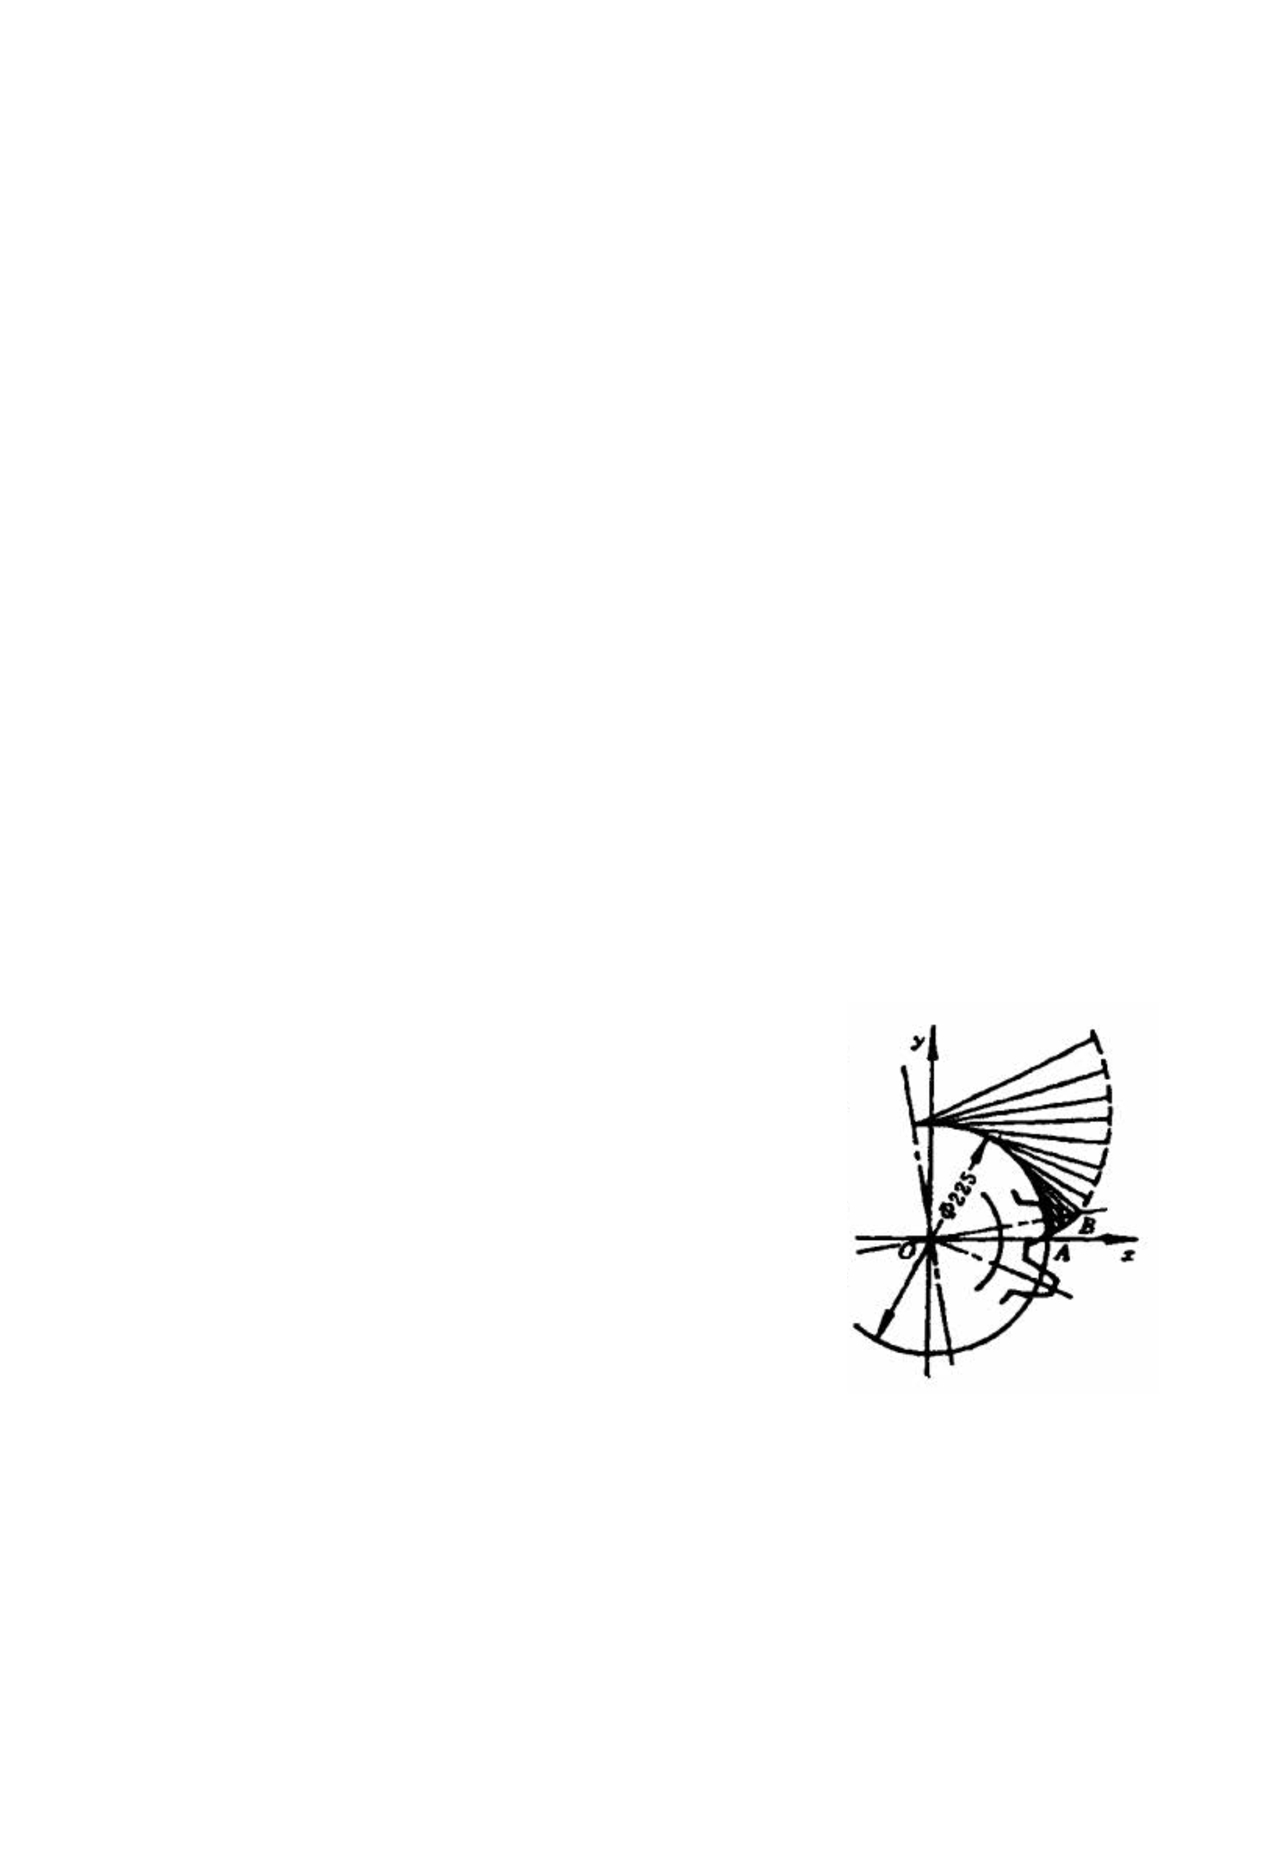
\includegraphics[scale=.7]{fig/6-7.pdf}
    \captionof*{figure}{第7题}
 \end{minipage}\hfill
 \begin{minipage}{.47\textwidth}
     \centering
 \begin{tikzpicture}[>=stealth]
   \draw[->](-2.75,0)--(2.75,0)node[below]{$x$};
   \draw[->](0,-2)--(0,2)node[left]{$y$};
 \node[below left]{$O$};
 \draw[thick](0,0)ellipse(2 and 1);
 \tkzDefPoints{1.5/0/P, 1/.866/Q}
 \draw(P)node[below]{$P$}--(Q)node[above]{$Q$};
\tkzDefMidPoint(P,Q) \tkzGetPoint{M}
\tkzLabelPoints[left](M) 
\tkzDrawPoints(M)
 \end{tikzpicture}    
 \captionof*{figure}{第9题}
 \end{minipage}
 
 


 \item 如图，已知椭圆$\frac{x^2}{a^2}+\frac{y^2}{b^2}=1\; (a>b>0)$，线段$QP$的长等于短半轴长，$Q$在椭圆上沿第一象限内的椭圆弧运动，$P$同时沿$x$轴滑动，并保持$Q$在$P$的左边. 求$QP$中点$M$的
 轨迹方程.
 \item P是椭圆$\frac{x^2}{a^2}+\frac{y^2}{b^2}=1\; (a>b>0)$上的点，过$A(-a,0)$, $A'(a,0)$分别作$PA$、$PA'$的垂线交于$Q$，当$P$在椭圆上运动时，求$Q$点的轨迹方程.
\item  已知$P(-2,2)$, $Q(0,2)$. 长为$\sqrt{2}$的线段$AB$在直线$x-y=0$上滑动. 设直线$PA$与$QB$交于$M$（如图），求点$M$的轨迹方程.

\noindent
\begin{minipage}{.4\textwidth}
\centering
\begin{tikzpicture}[>=stealth, scale=.6]
    \draw[->](-4,0)--(2.75,0)node[below]{$x$};
    \draw[->](0,-4)--(0,3)node[left]{$y$};
  \node[below right]{$O$};
\draw[domain=-3.5:2, thick]plot(\x, \x);
\tkzDefPoints{-2/2/P, 0/2/Q, -.25/-.25/B, -1.25/-1.25/A}
\tkzInterLL(P,A)(Q,B)  \tkzGetPoint{M}
\tkzDrawPoints(P,Q)
\tkzDrawSegments[very thick](A,B)
\tkzDrawSegments[thick](P,M)
\tkzDrawLines[add=0 and .2](Q,M)
\tkzLabelPoints[left](A,B,P)
\tkzLabelPoints[right](Q,M)

\end{tikzpicture}    
   \captionof*{figure}{第11题}
\end{minipage}\hfill
\begin{minipage}{.57\textwidth}
    \centering
\begin{tikzpicture}[>=stealth]
  \draw[->](-2.75,0)--(3.5,0)node[below]{$x$};
  \draw[->](0,-2)--(0,2)node[left]{$y$};
\node[below left]{$O$};
\draw[thick](0,0)ellipse(2 and 1);
\tkzDefPoints{ 1.5/-.66/C, 1.5/.66/B, 2/0/A, -2/0/A_1}
\tkzInterLL(A_1,B)(C,A) \tkzGetPoint{P}
\tkzDrawLines[add=0 and .4](A_1,B C,P)
\tkzDrawLines[add=.4 and .4](B,C)
\tkzLabelPoints[below left](A_1)
\tkzLabelPoints[above right](B)
\tkzLabelPoints[below right](C,A)
\tkzLabelPoints[above left](P)
\tkzDrawPoints(P)
\end{tikzpicture}    
\captionof*{figure}{第12题}
\end{minipage}

\item 如图，已知椭圆$\frac{x^2}{a^2}+\frac{y^2}{b^2}=1\; (a>b>0)$，长轴两端点为$A_1(-a,0)$和$A(a,0)$，直线$BC\bot x$轴，交椭圆于$B$、$C$. 求直线$A_1B$与$CA$的交点$P$的轨迹方程.
\item 求证：椭圆$\frac{x^2}{a^2}+\frac{y^2}{b^2}=1\; (a>b>0)$
上的三点对于同一焦点的焦半径成等差数列的充要条件是该三点的横坐标成等差数列.
\item 平行四边形的两边分别在某双曲线的两条渐近线上，一个顶点在双曲线上，求证此平行四边形的面积是定值.
\item 抛物线$y^2=2px\; (p>0)$上有点$P$，$P$在$x$轴上的射影为$M$，$N$是$PM$中点，$NQ\parallel x$轴，$NQ$交抛物线于$Q$，直线$MQ$交$y$轴于$T$，

求证：$3|OT|=2|PM|$
\item 已知椭圆$\frac{x^2}{a^2}+\frac{y^2}{b^2}=1\; (a>b>0)$和圆$x^2+y^2=b^2$，$P$是椭圆上非短轴端点的任意一点，过$P$作圆的切线，$Q$、$R$为切点，直线$QR$分别交$x$轴和$y$轴于$S$、$T$. 

求证$\frac{b^2}{|OS|^2}+\frac{a^2}{|OT|^2}$为定值.
\item 已知直线$\frac{x}{a}+\frac{y}{b}=1$，求证：
\begin{enumerate}[(1)]
\item 若$\frac{1}{a}+\frac{1}{b}$为定值，则直线恒过定点；
\item 若$\frac{1}{a^2}+\frac{1}{b^2}$为定值，则直线恒与定圆相切.
\end{enumerate}

\item 已知曲线$xy=m^2\; (x,y\in\R^+)$，直线$\ell$与它交于$B$、$C$，与两坐标轴交于$A$、$D$. 求证：
\begin{enumerate}[(1)]
\item $|AB|=|CD|$;
\item 若曲线将线段$AD$三等分，则$\triangle OAD$的面积为定值（$O$为坐标原点）.
\end{enumerate}

\item 过定点$M(-1,3)$引直线交抛物线$y^2=16x$于$A$、$B$两点. 求$|AM|\cdot |BM|$的最小值.
\item 已知椭圆$\frac{x^2}{16}+\frac{y^2}{25}=1$，且点$A$横坐标为4，点$C$纵坐标为5，求椭圆的内接四边形$ABCD$的最大面积．

\item 设椭圆左顶点在抛物线$y^2=x-1$上，长轴长为4，左准线为$y$轴.
\begin{enumerate}[(1)]
\item 求上述椭圆中心的轨迹方程；
\item 求其中离心率最大的椭圆．
\end{enumerate}

\end{enumerate}
